\documentclass{article}

\usepackage{ctex}
\usepackage{graphicx}
\usepackage{amsmath}
\usepackage{cite}
\usepackage{subfigure}
\usepackage{booktabs}

\usepackage[left=2.5cm, right=2.5cm, top=2.8cm, bottom=2.8cm]{geometry}

\begin{document}

% \begin{figure}[htbp]
%     \subfigure[单放射源无屏蔽空间]{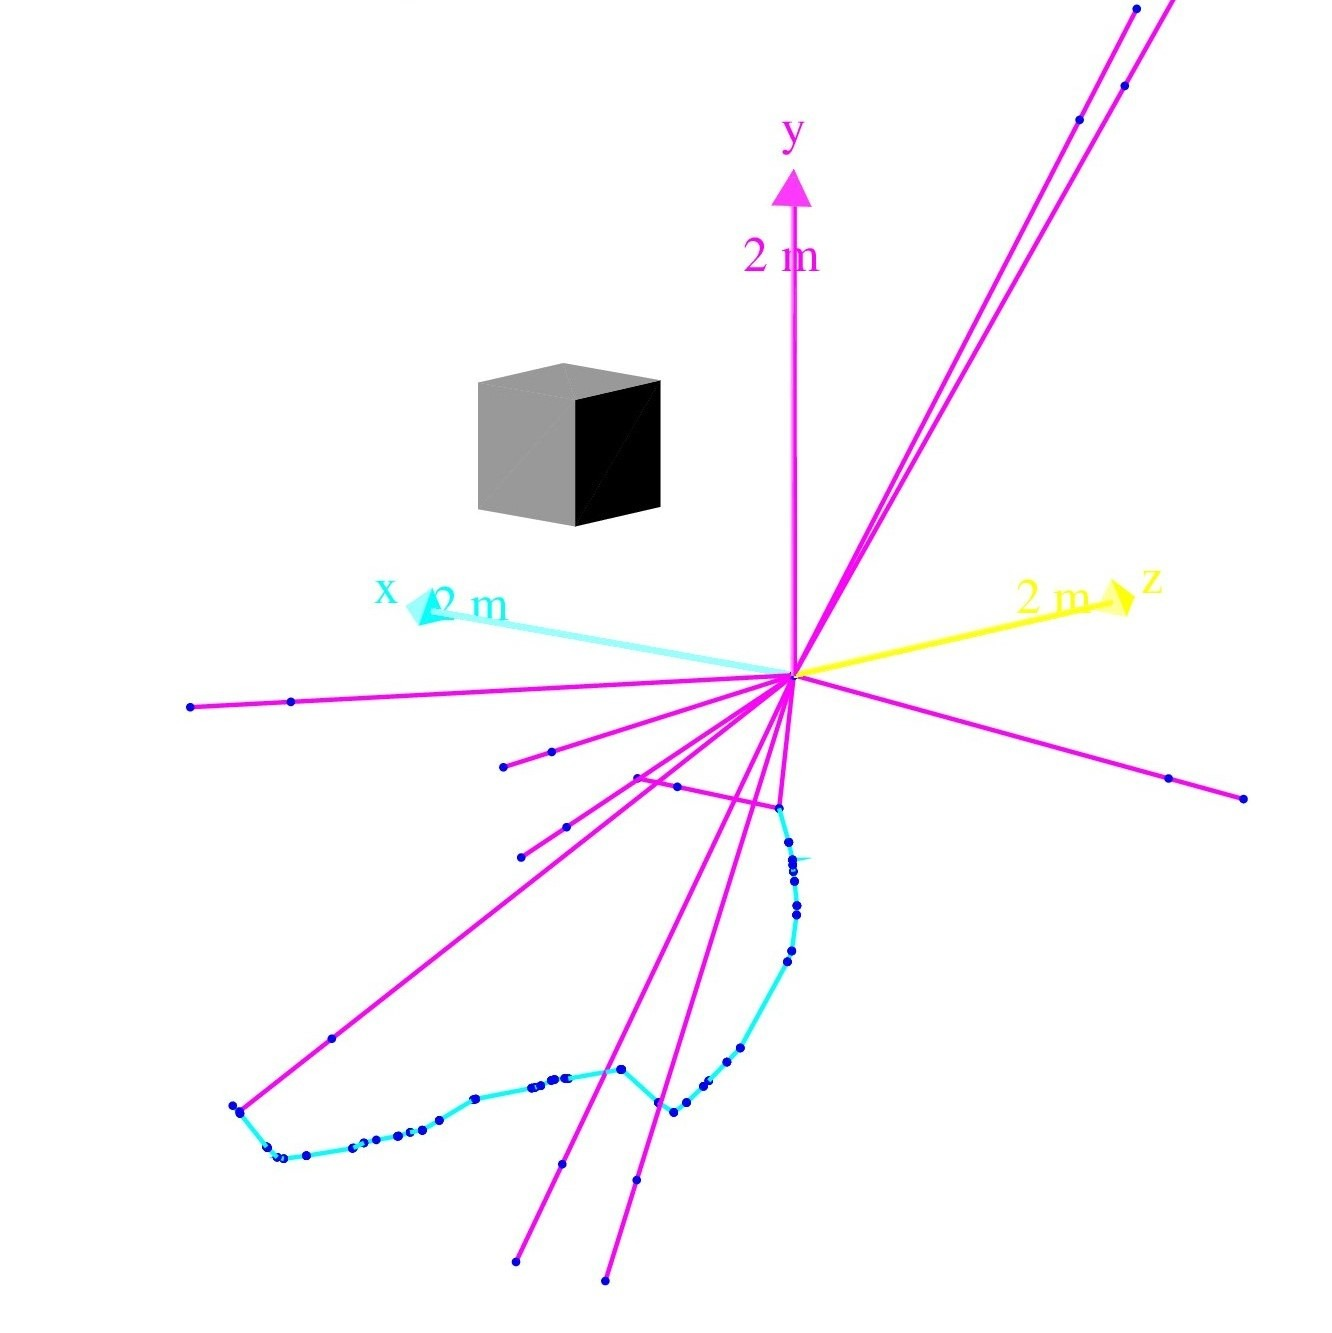
\includegraphics[width=0.45\textwidth]{figures/SingleSource.jpg}\label{fig:exph1}}
%     \subfigure[多放射源无屏蔽空间]{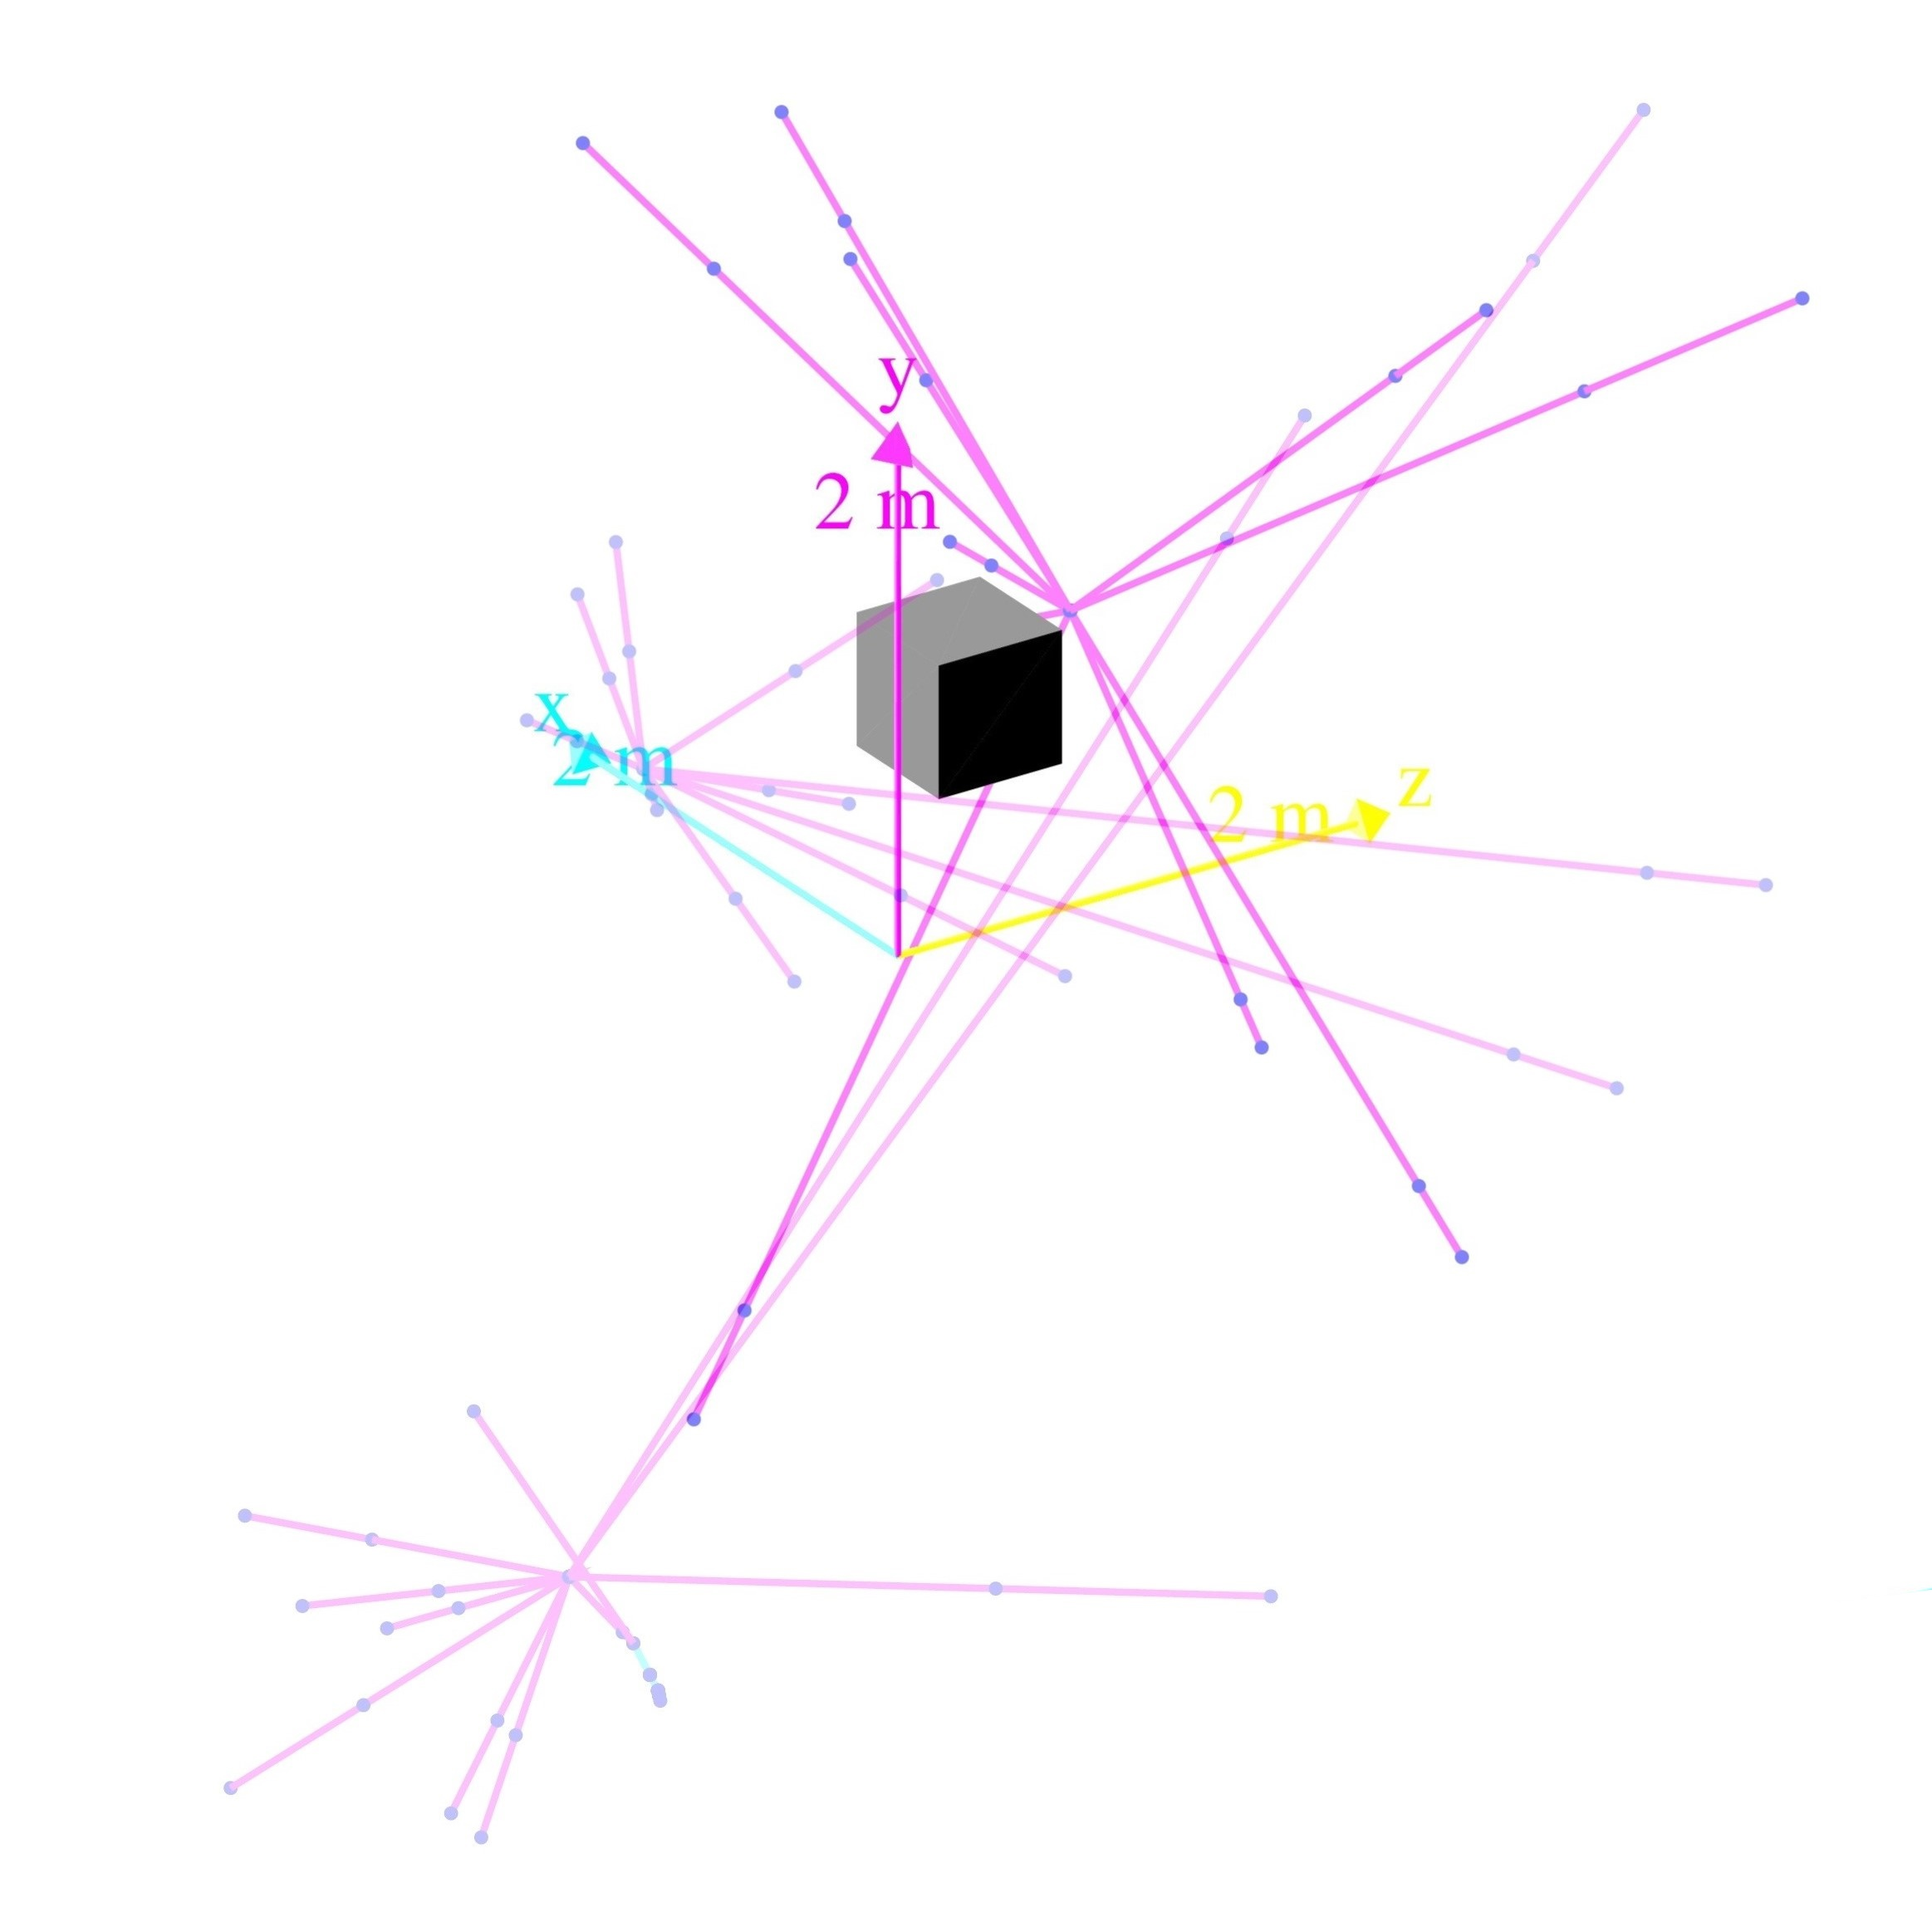
\includegraphics[width=0.45\textwidth]{figures/MultiSources.jpg}\label{fig:exgr1}}
%     \caption{Geant4模拟单源辐射场和多源辐射场}
%     \label{Geant4模拟单源辐射场和多源辐射场}
% \end{figure}

% \begin{figure}[htbp]
%     \subfigure[单放射源无屏蔽辐射场剂量分布]{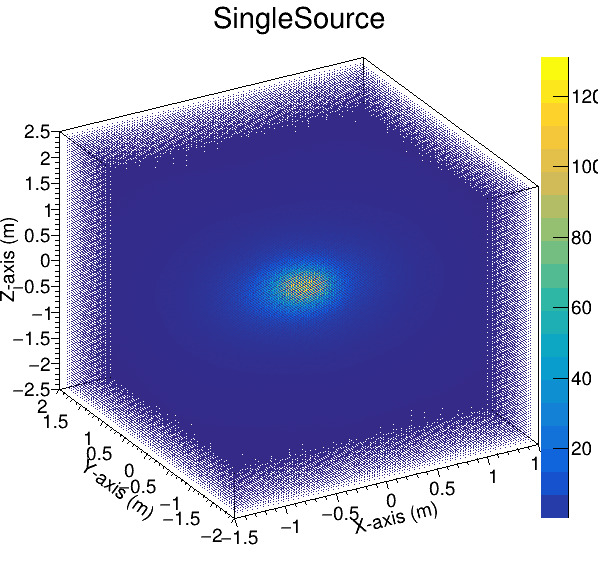
\includegraphics[width=0.45\textwidth]{figures/SingleSource.png}\label{fig:exph2}}
%     \subfigure[多放射源无屏蔽辐射场剂量分布]{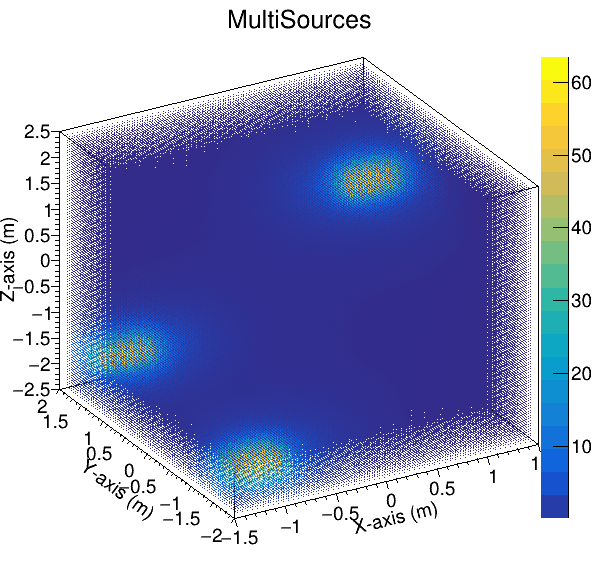
\includegraphics[width=0.45\textwidth]{figures/MultiSources.png}\label{fig:exgr2}}
%     \caption{Geant4模拟单源辐射场和多源辐射场的剂量分布}
%     \label{Geant4模拟单源辐射场和多源辐射场的剂量分布}
% \end{figure}

% \begin{figure}[htbp]
%     \subfigure[单放射源无屏蔽空间]{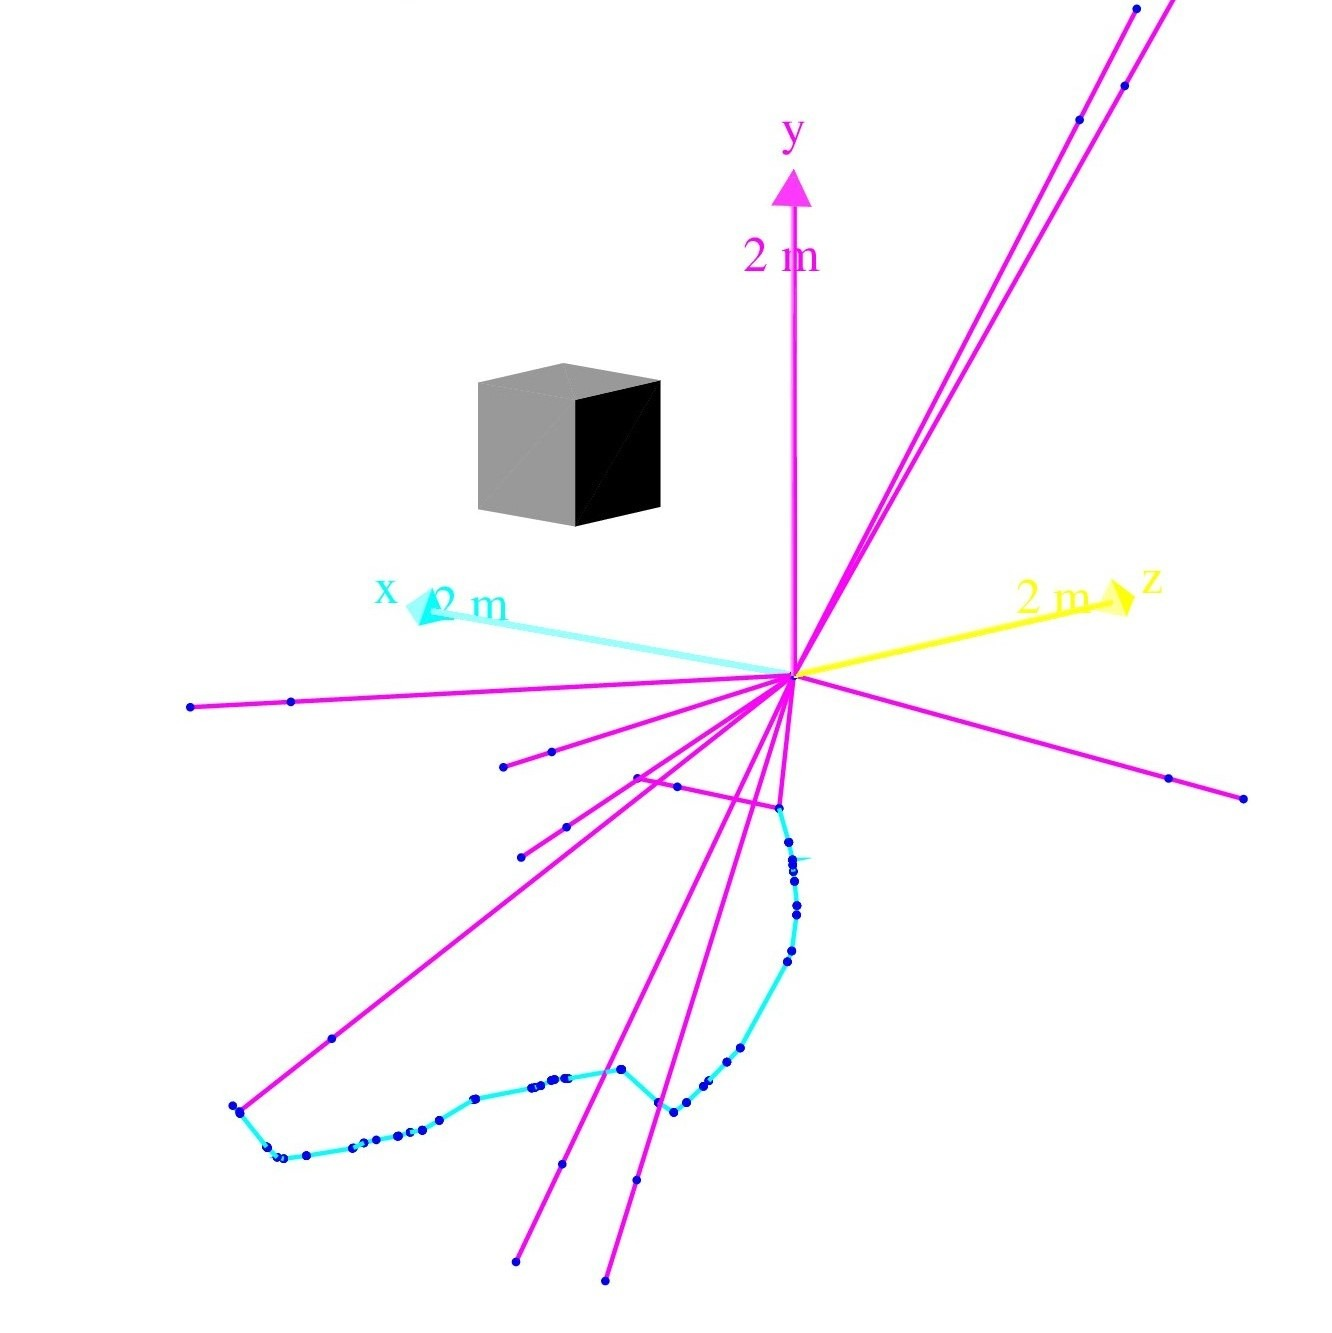
\includegraphics[width=0.45\textwidth]{figures/SingleSource.jpg}\label{fig:exph3}}
%     \subfigure[单放射源有屏蔽空间]{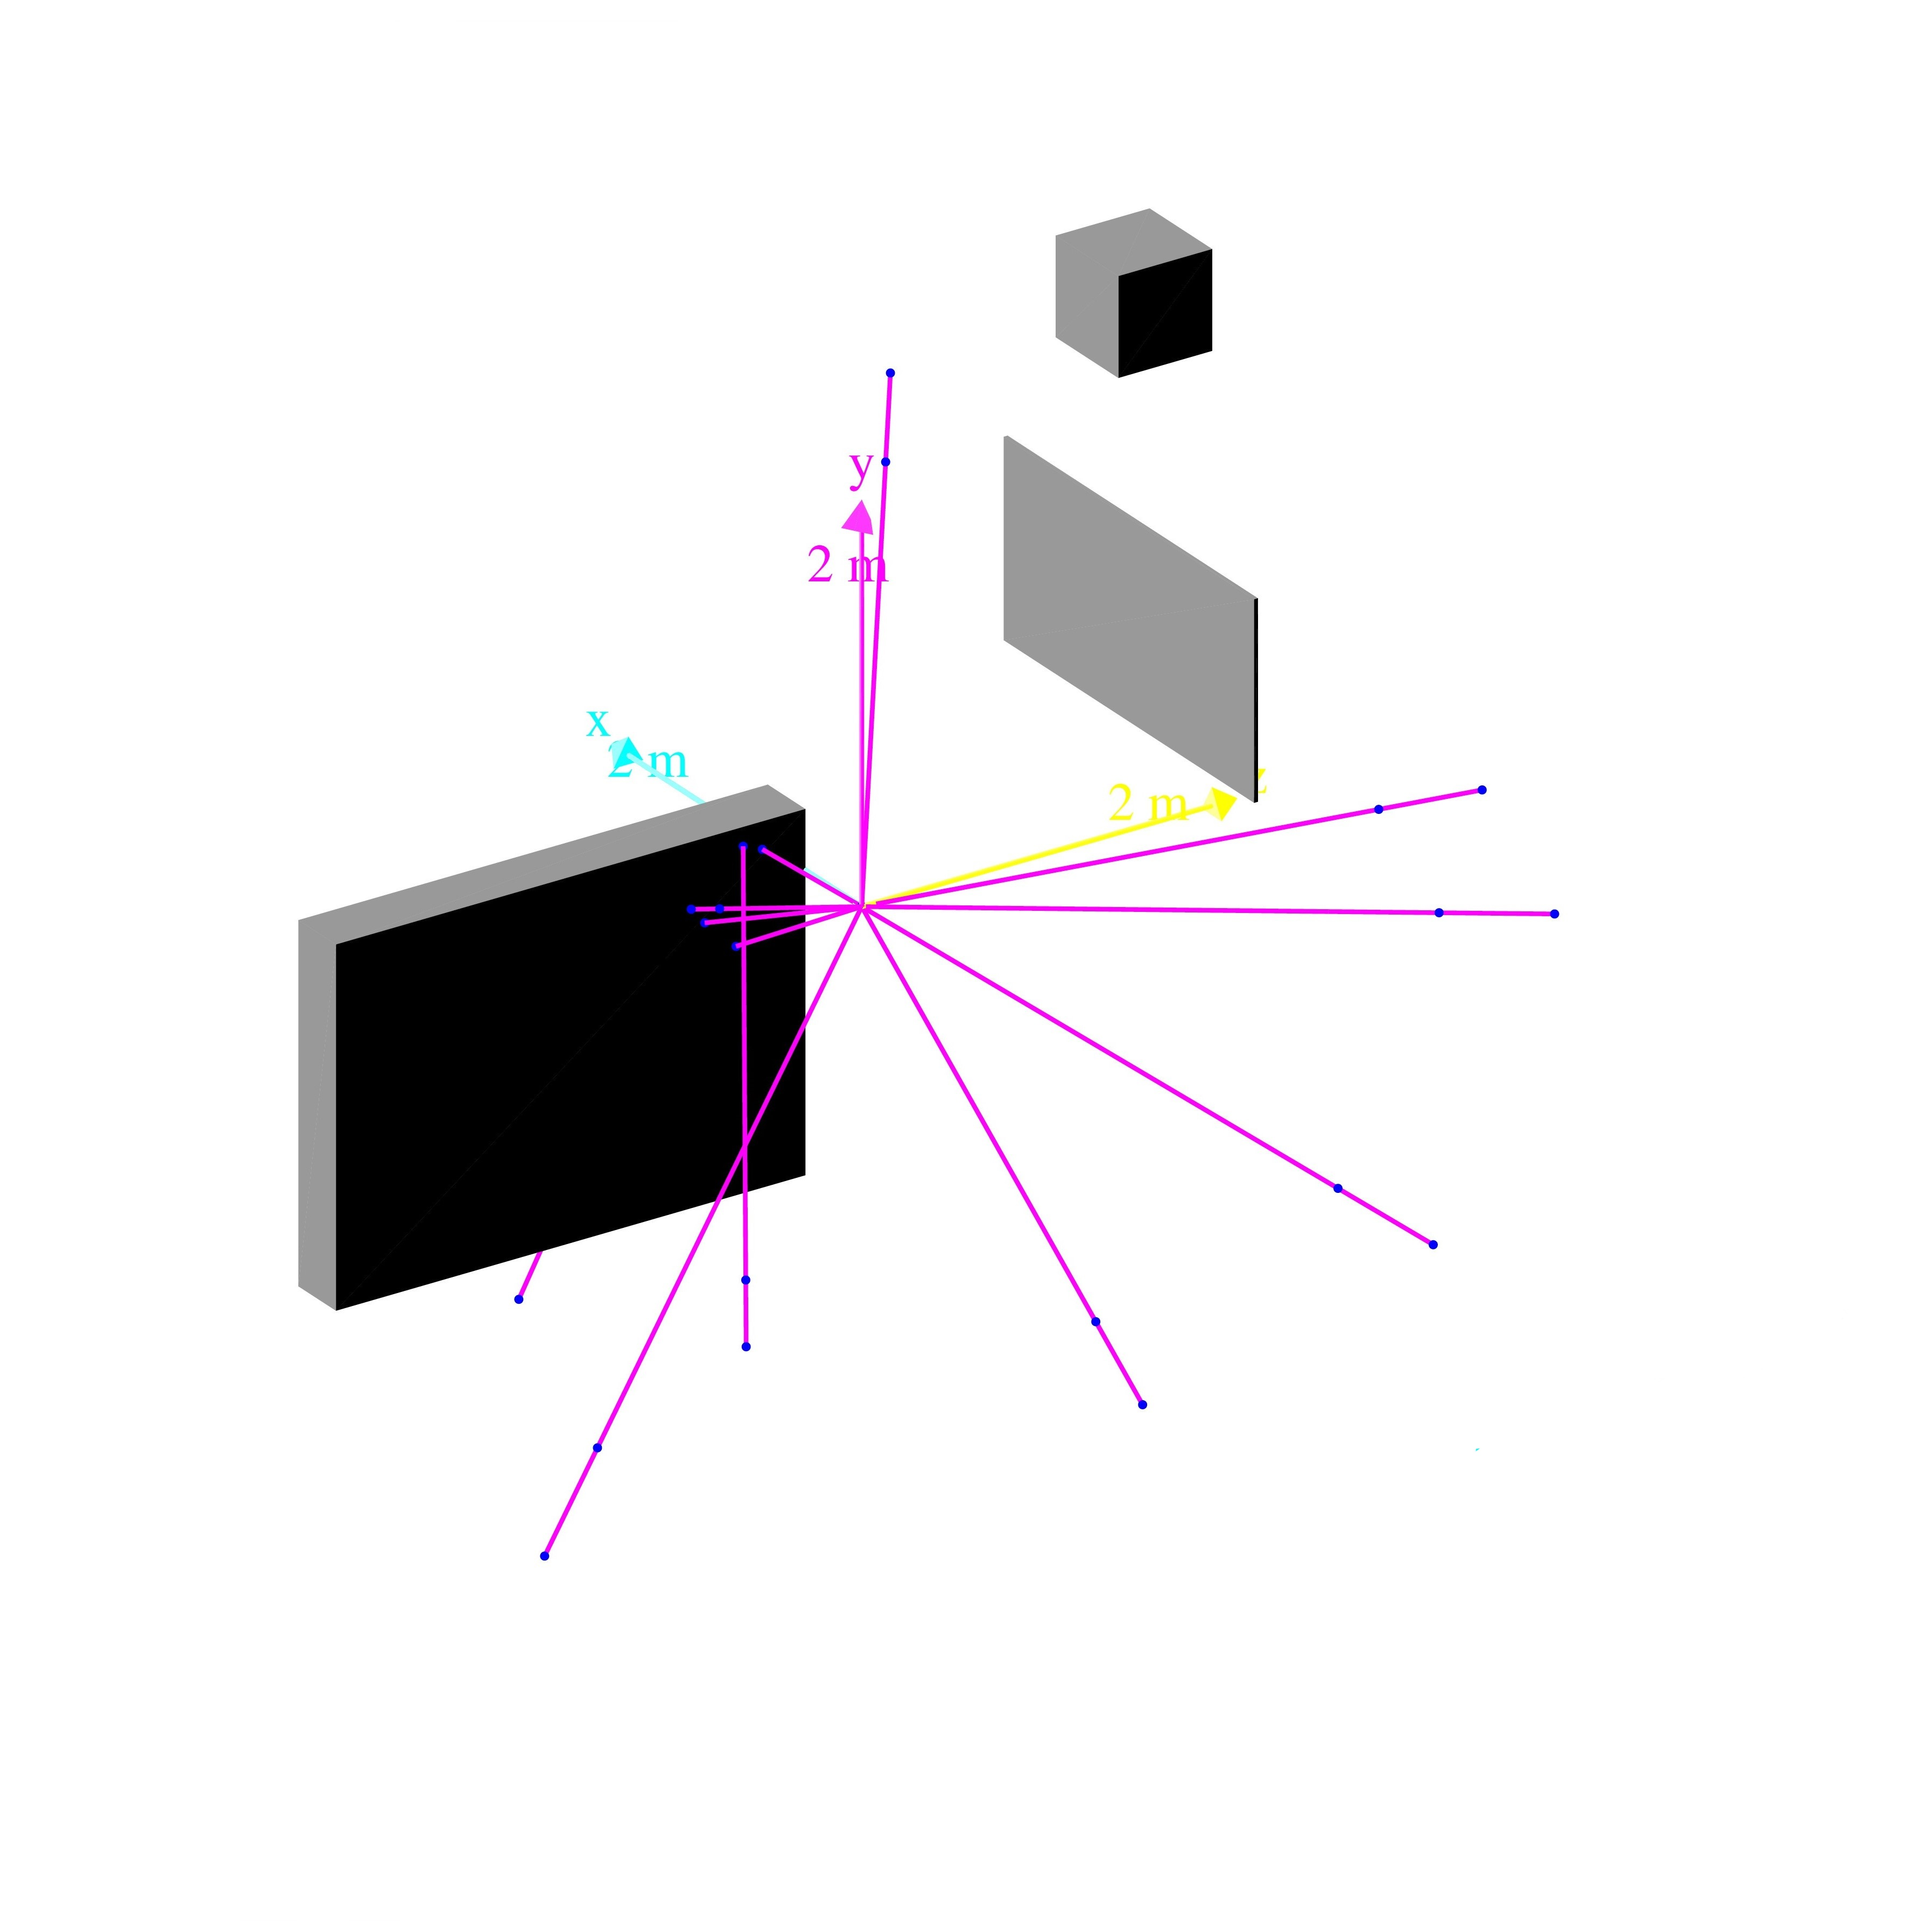
\includegraphics[width=0.45\textwidth]{figures/SingleSourceShield.jpg}\label{fig:exgr3}}
%     \caption{Geant4模拟无屏蔽空间辐射场和有屏蔽空间辐射场}
%     \label{Geant4模拟无屏蔽空间辐射场和有屏蔽空间辐射场}
% \end{figure}

% \begin{figure}[htbp]
%     \subfigure[单点源无屏蔽辐射场剂量分布]{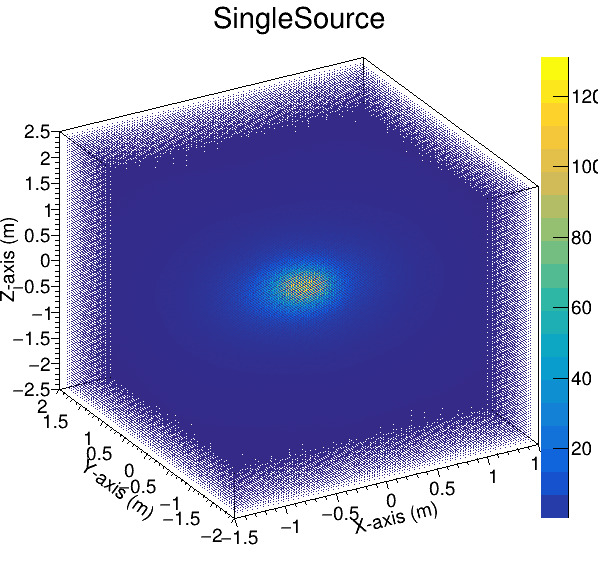
\includegraphics[width=0.45\textwidth]{figures/SingleSource.png}\label{fig:exph4}}
%     \subfigure[单点源有屏蔽辐射场剂量分布]{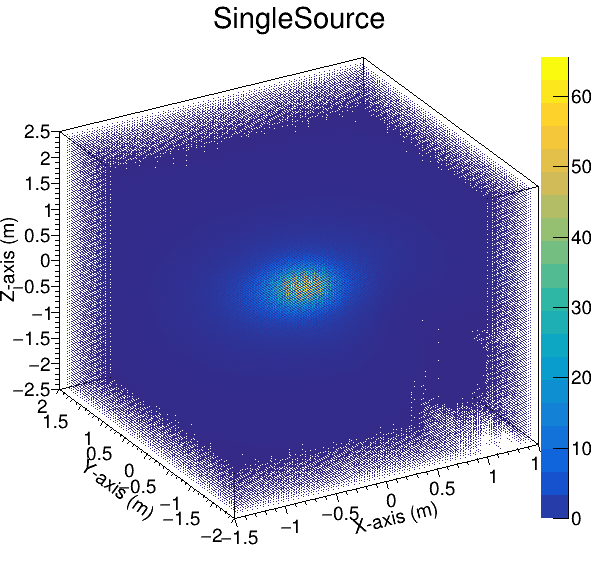
\includegraphics[width=0.45\textwidth]{figures/SingleSoourceShielded.png}\label{fig:exgr4}}
%     \caption{Geant4模拟单点源无屏蔽辐射场和单点源有屏蔽辐射场的剂量分布}
%     \label{Geant4模拟无屏蔽辐射场和有屏蔽辐射场的剂量分布}
% \end{figure}

% \begin{figure}[htbp]
%     \centering
%     \subfigure[单点源无屏蔽空间场]{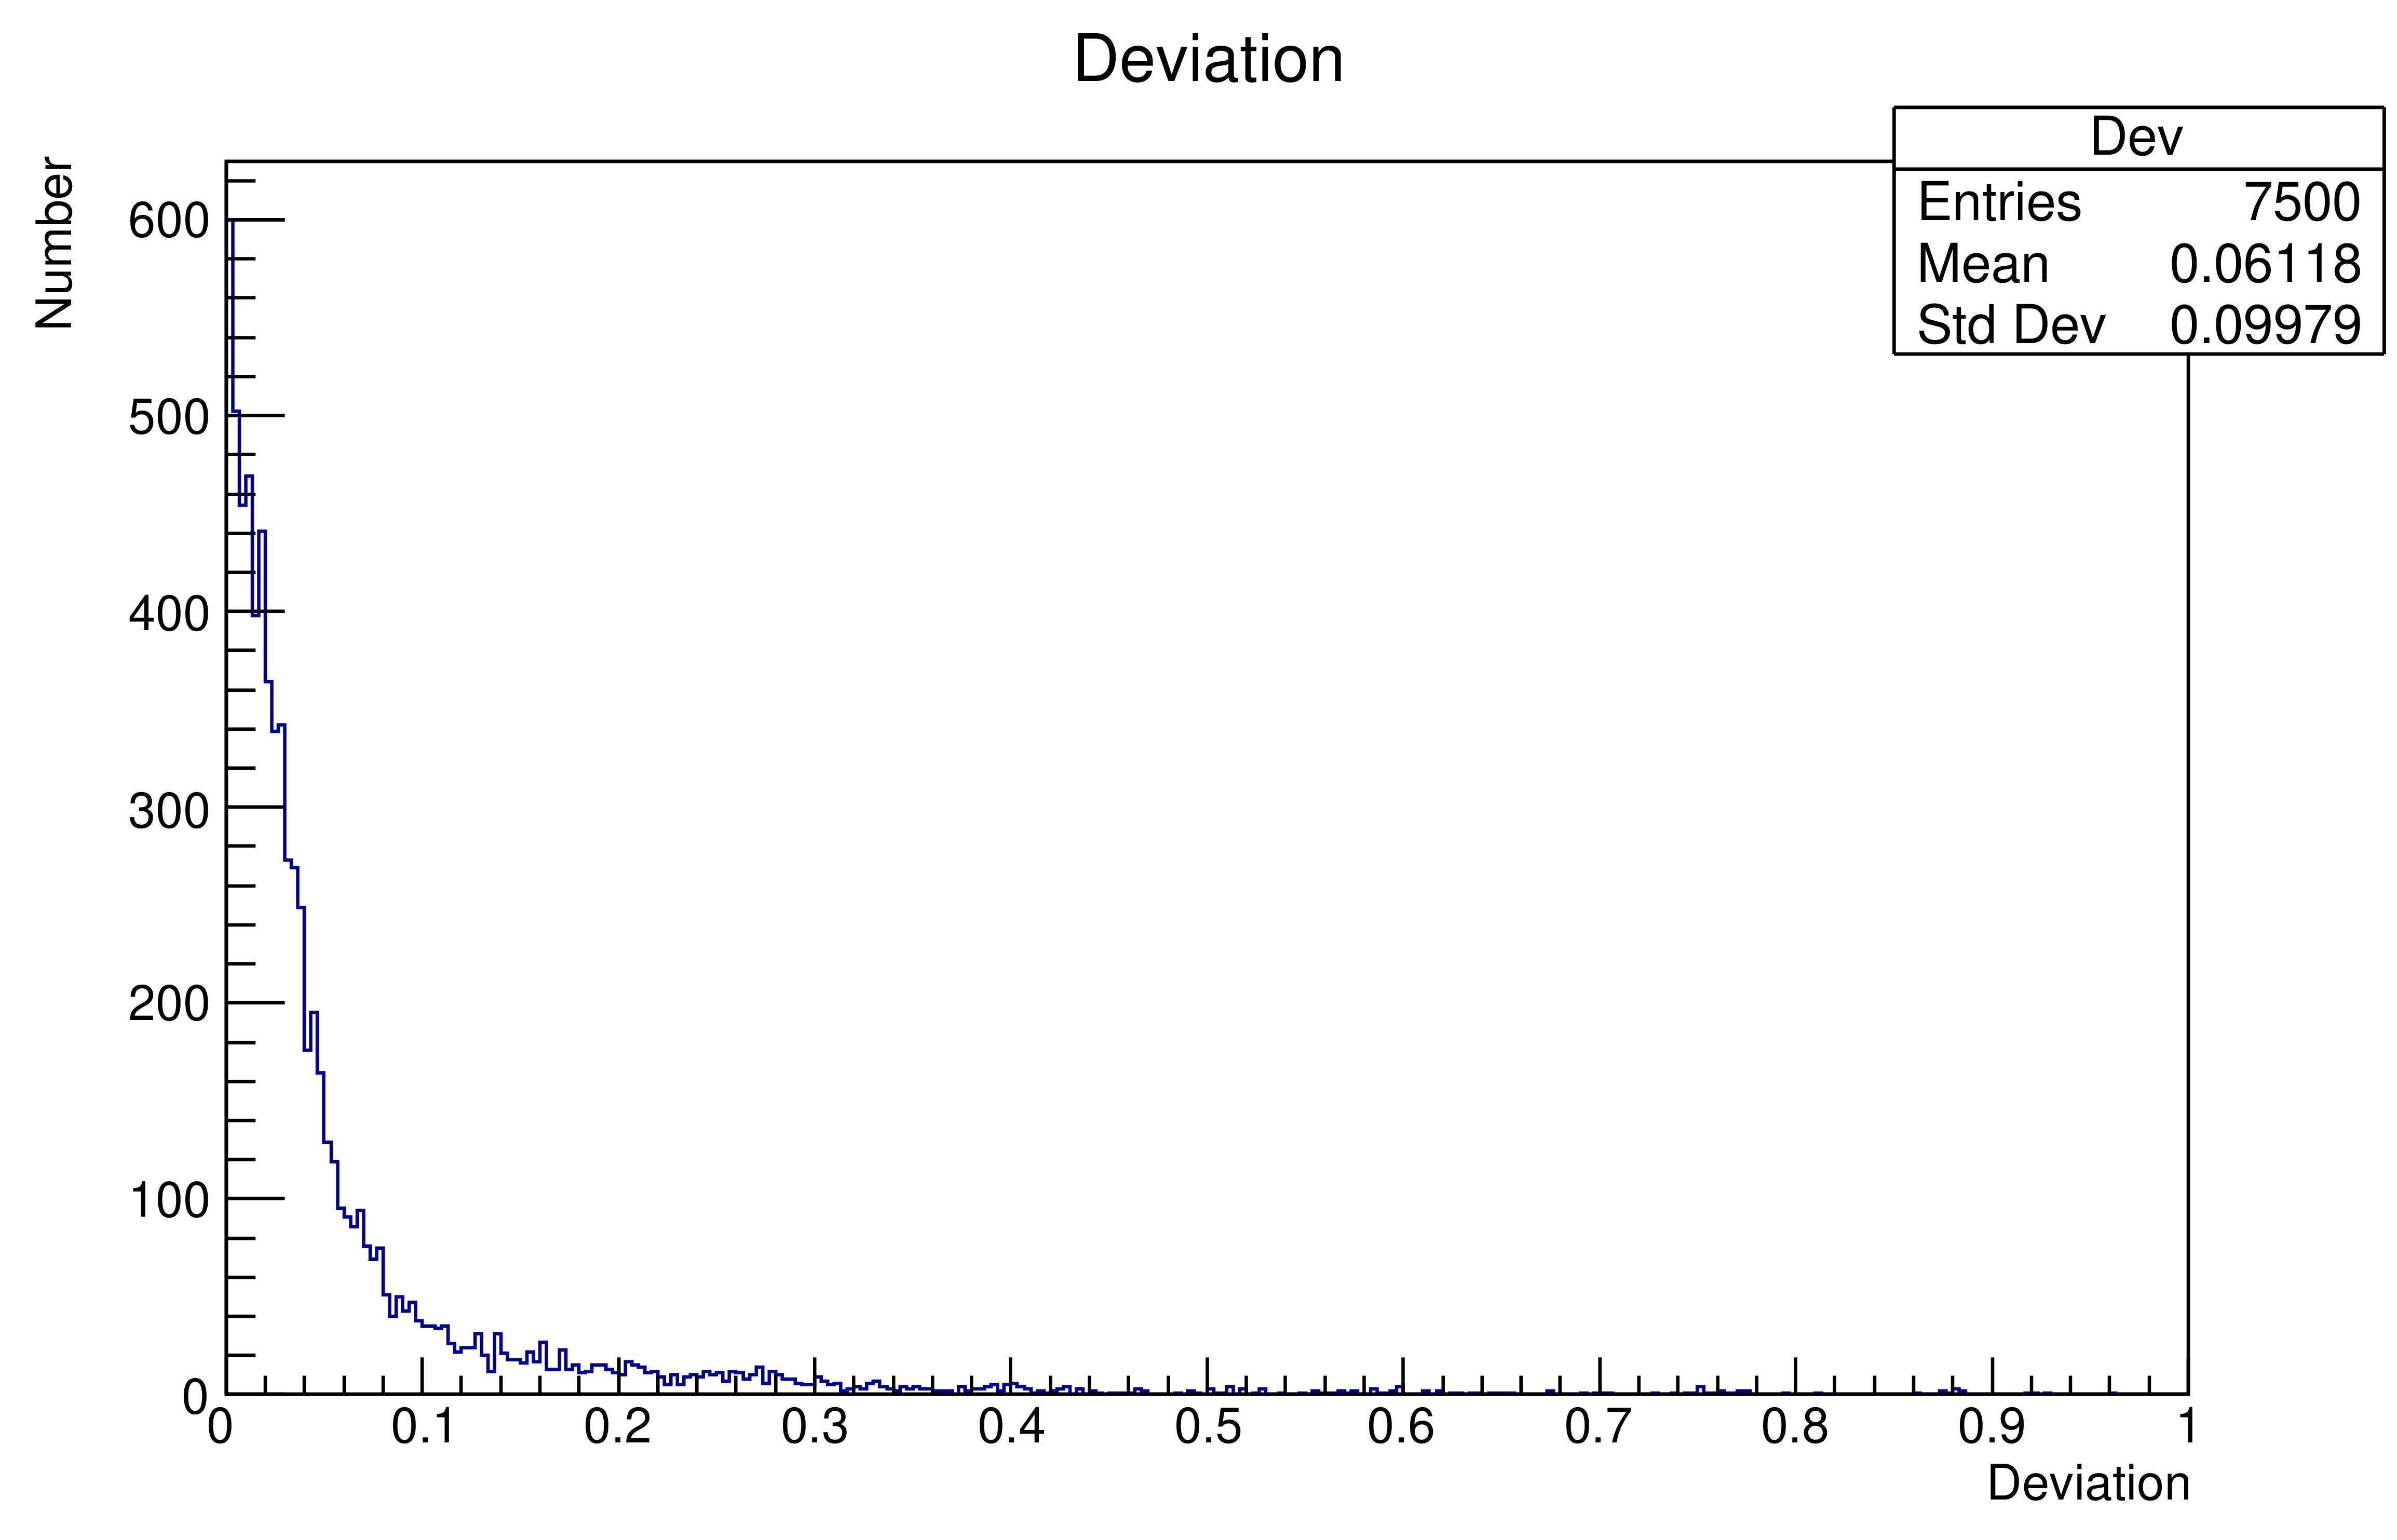
\includegraphics[width=0.45\textwidth]{figures/Deviation/SingleSourceUnshield.jpg}\label{fig:exph5}}
%     \subfigure[多点源无屏蔽空间场]{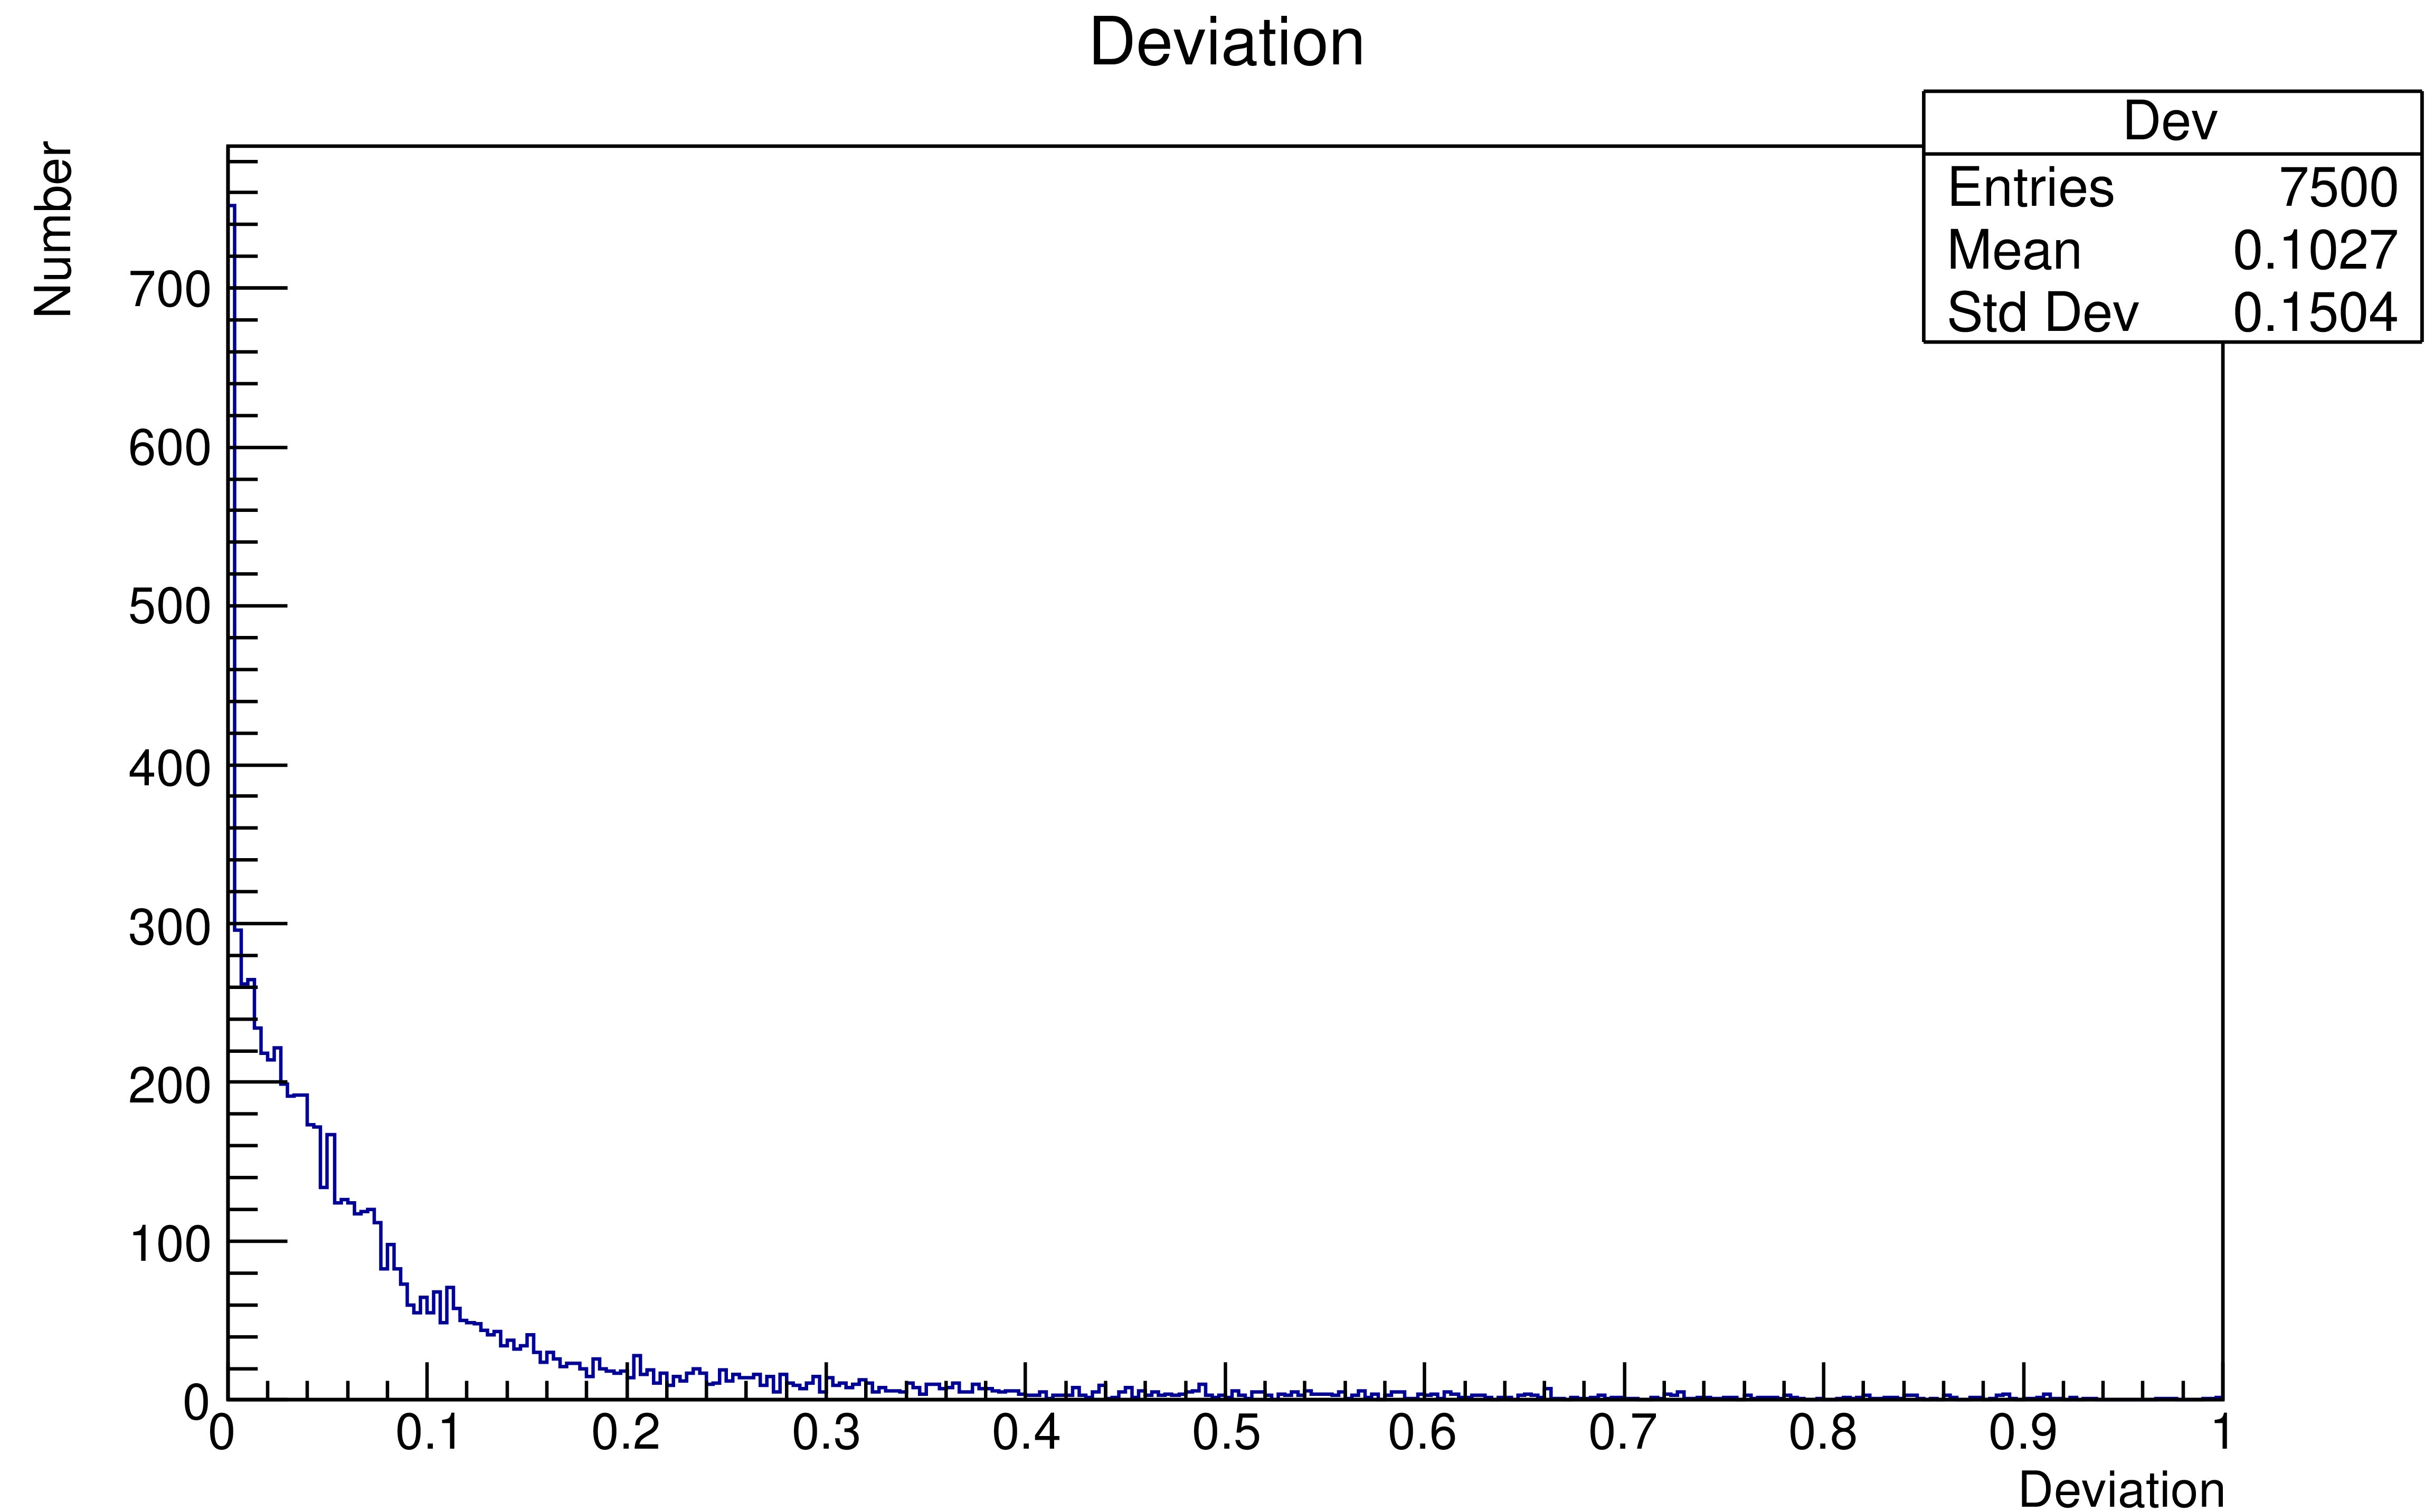
\includegraphics[width=0.45\textwidth]{figures/Deviation/MultiSourcesUnshield.jpg}\label{fig:exgr5}}

%     \subfigure[单点源无屏蔽空间场]{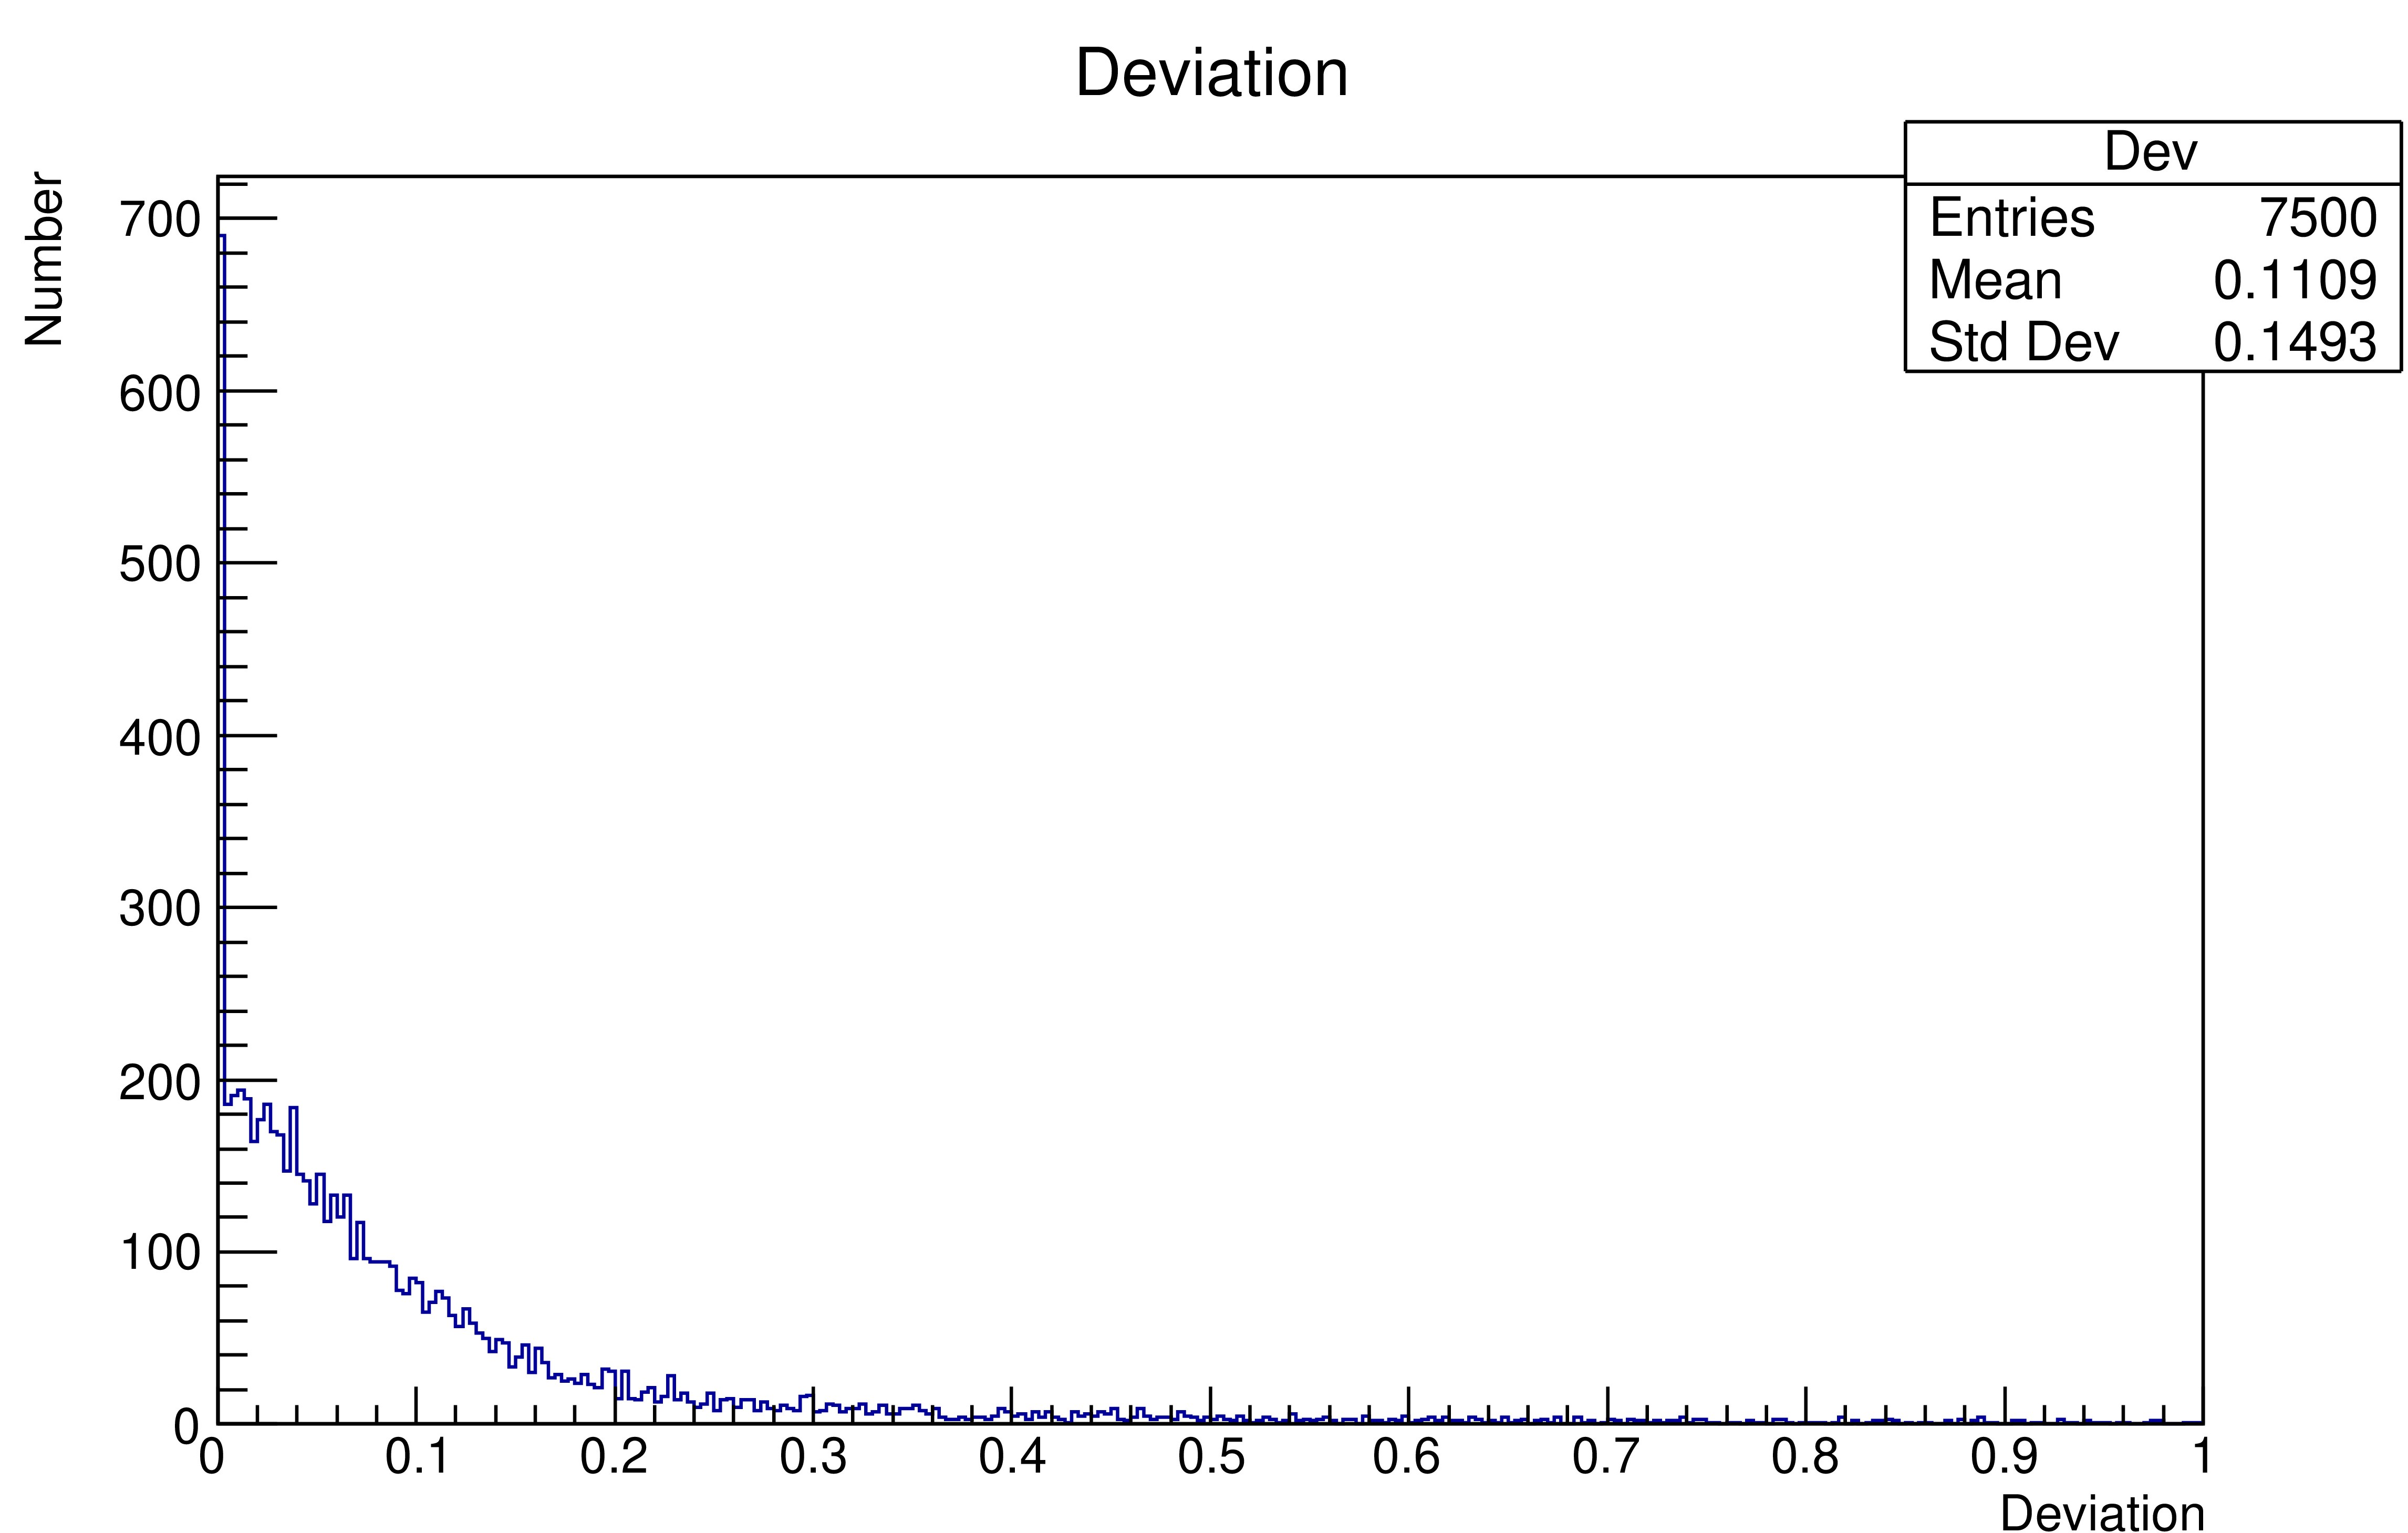
\includegraphics[width=0.45\textwidth]{figures/Deviation/SingleSourceShield.jpg}\label{fig:exph6}}
%     \subfigure[多点源有屏蔽空间场]{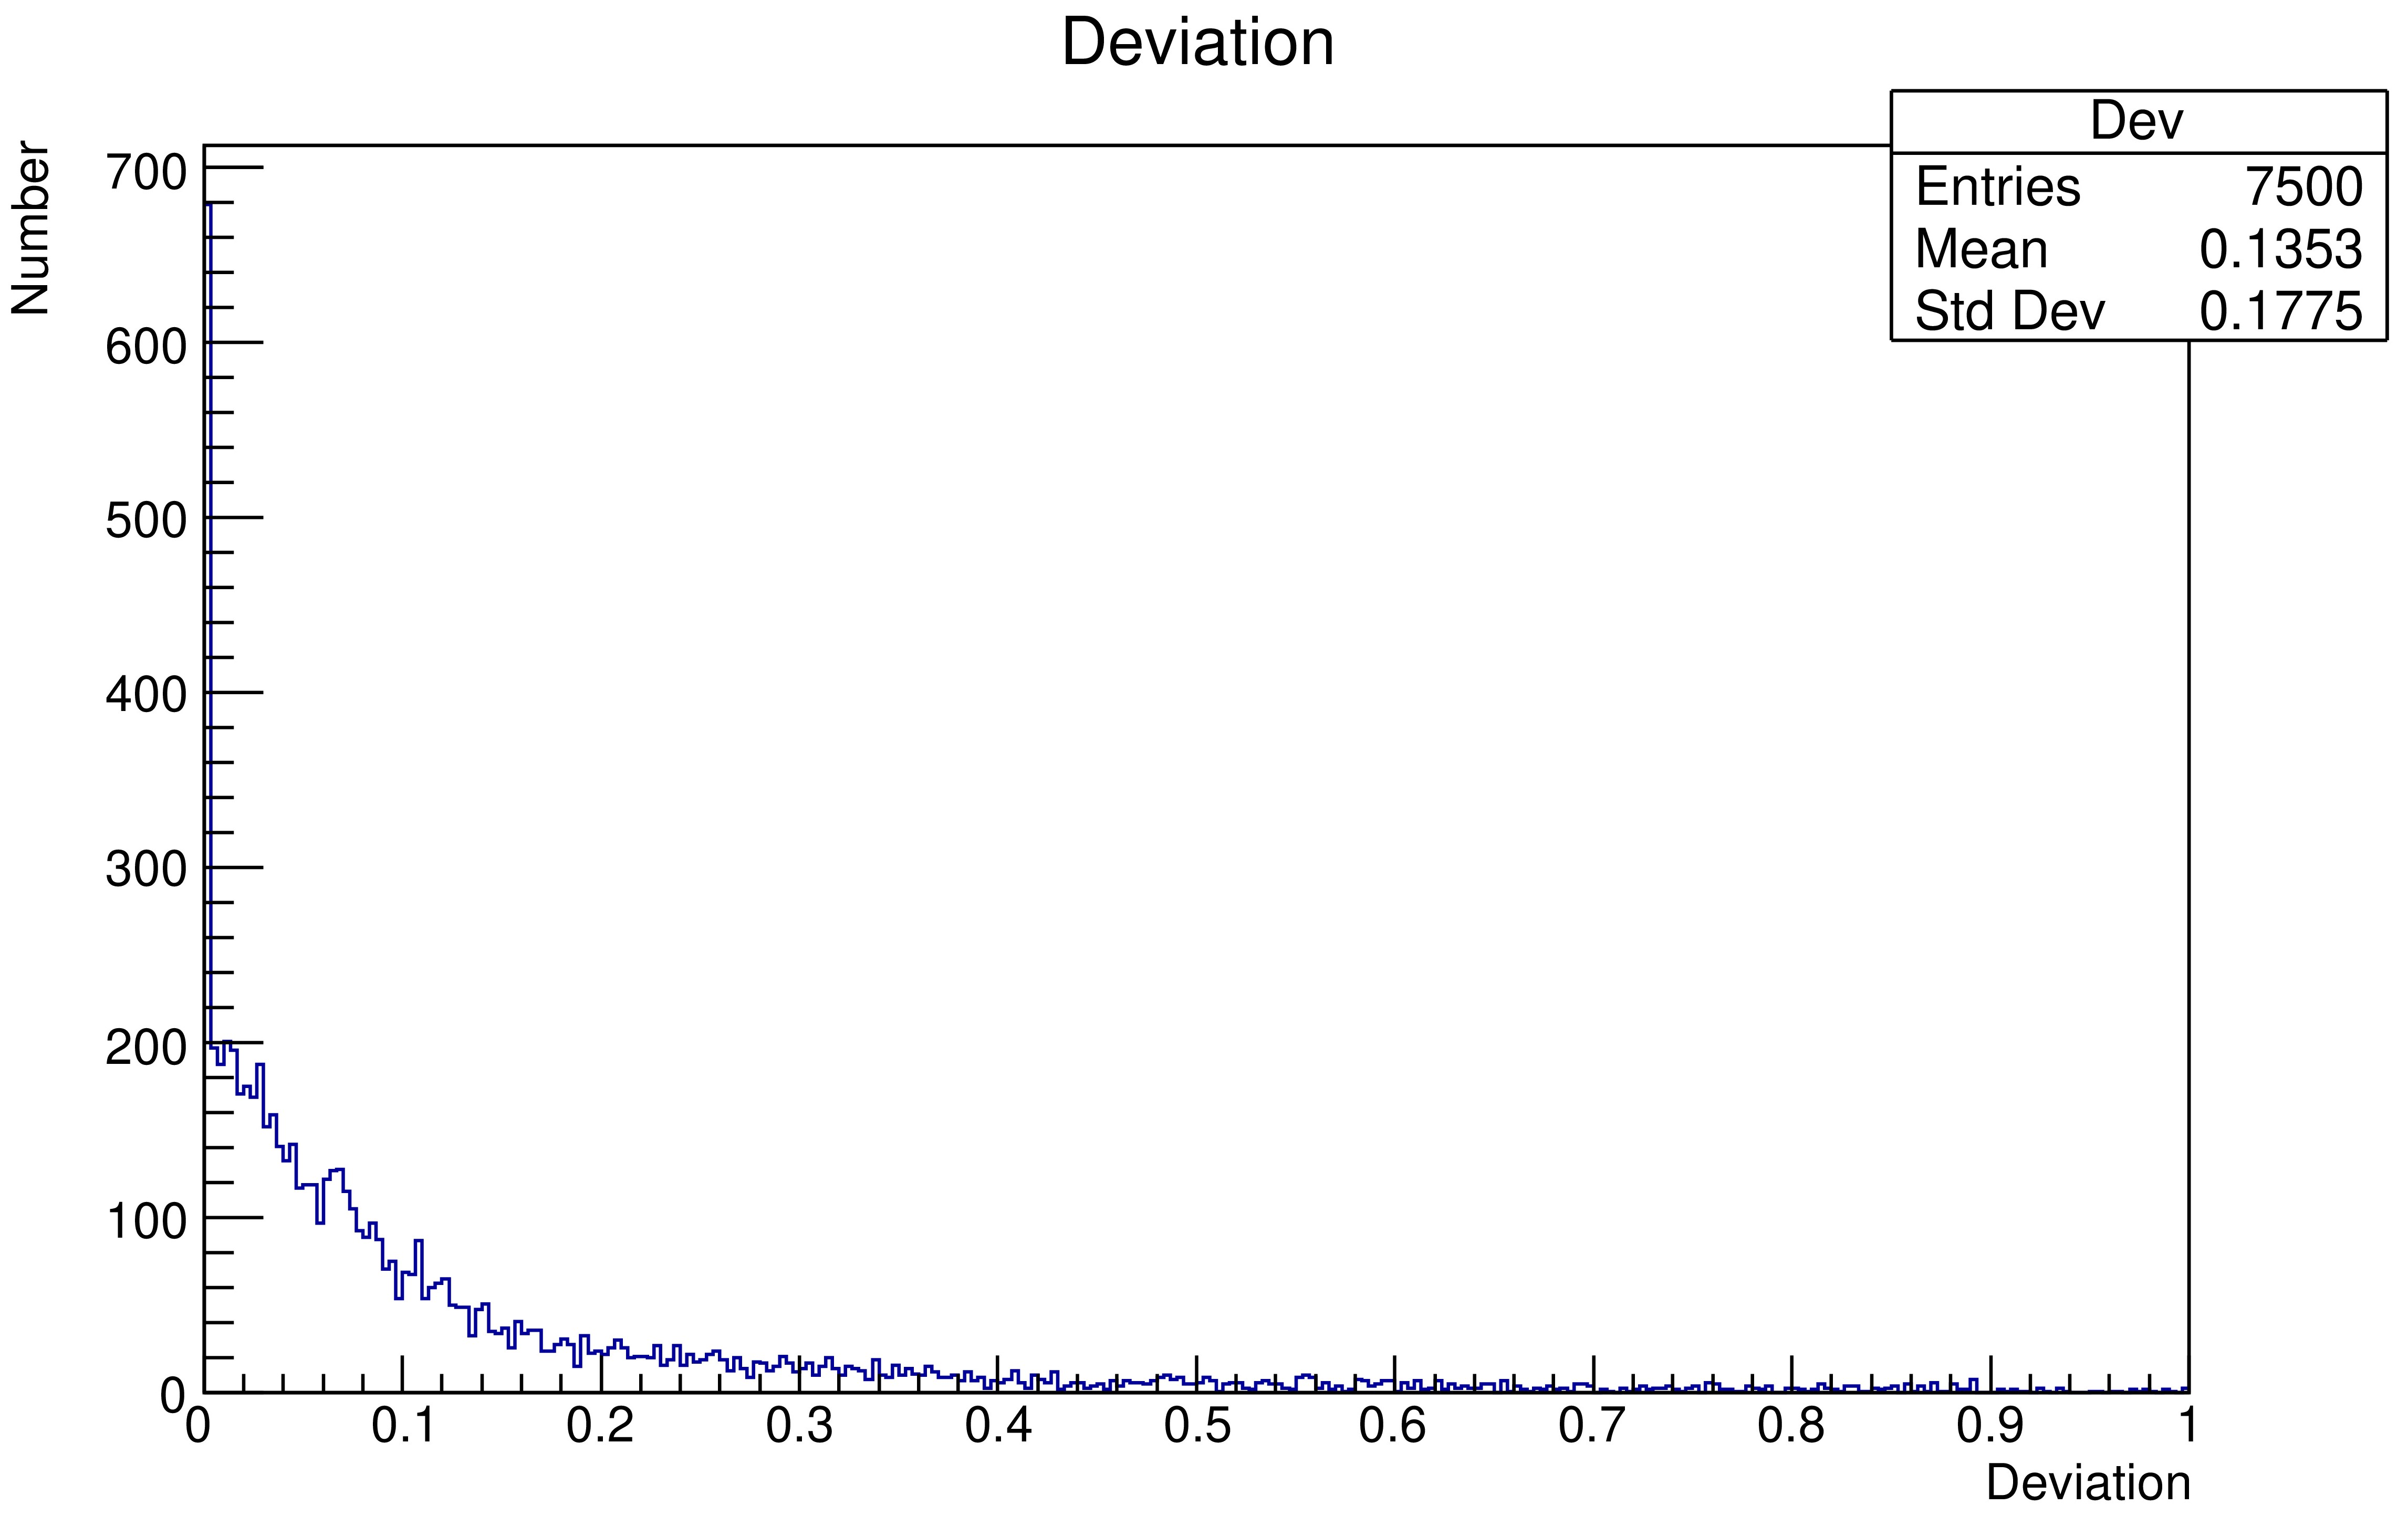
\includegraphics[width=0.45\textwidth]{figures/Deviation/MultiSourcesShield.jpg}\label{fig:exgr6}}

%     \caption{空间辐射场插值重构相对偏差分布}
%     \label{空间辐射场插值重构相对偏差分布}
% \end{figure}

% \begin{figure}[htbp]
%     \centering
%     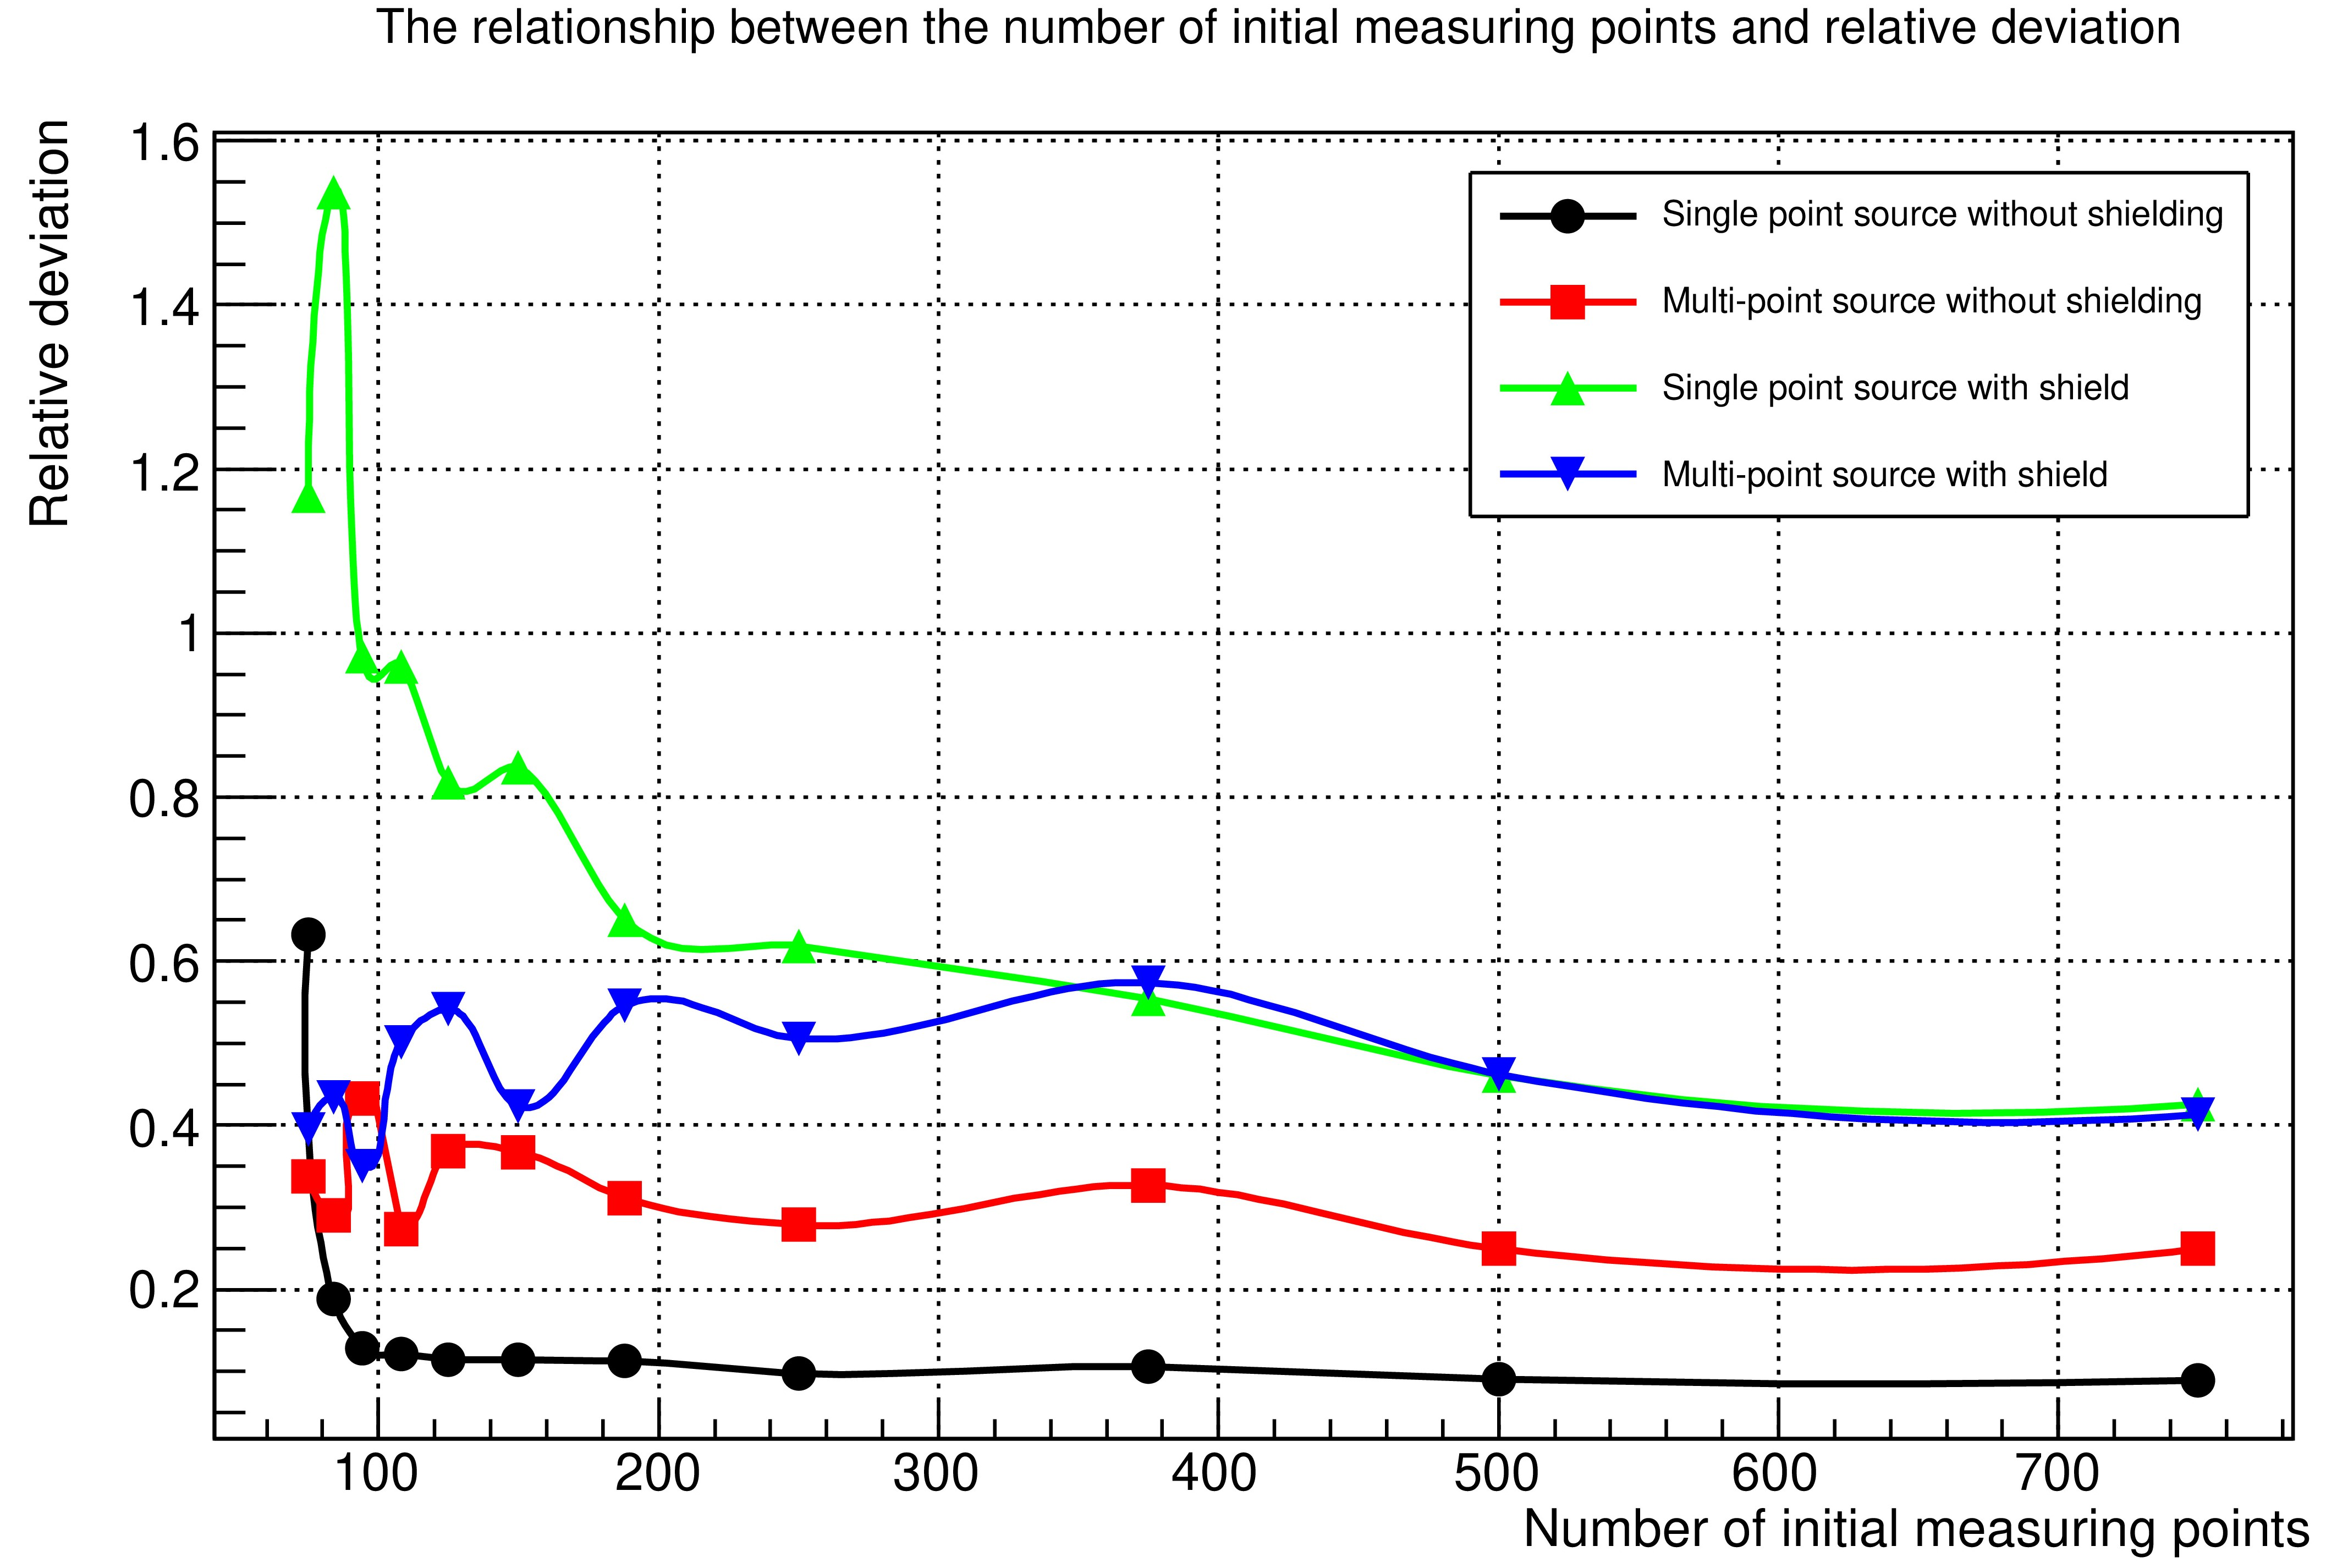
\includegraphics[width=0.8\textwidth]{figures/Deviation/MeasurePoints.jpg}
%     \caption{初始测点数量与相对偏差的关系}
%     \label{初始测点数量与相对偏差的关系}
% \end{figure}

% \begin{figure}[htbp]
%     \centering
%     \subfigure[多层B样条插值重构]{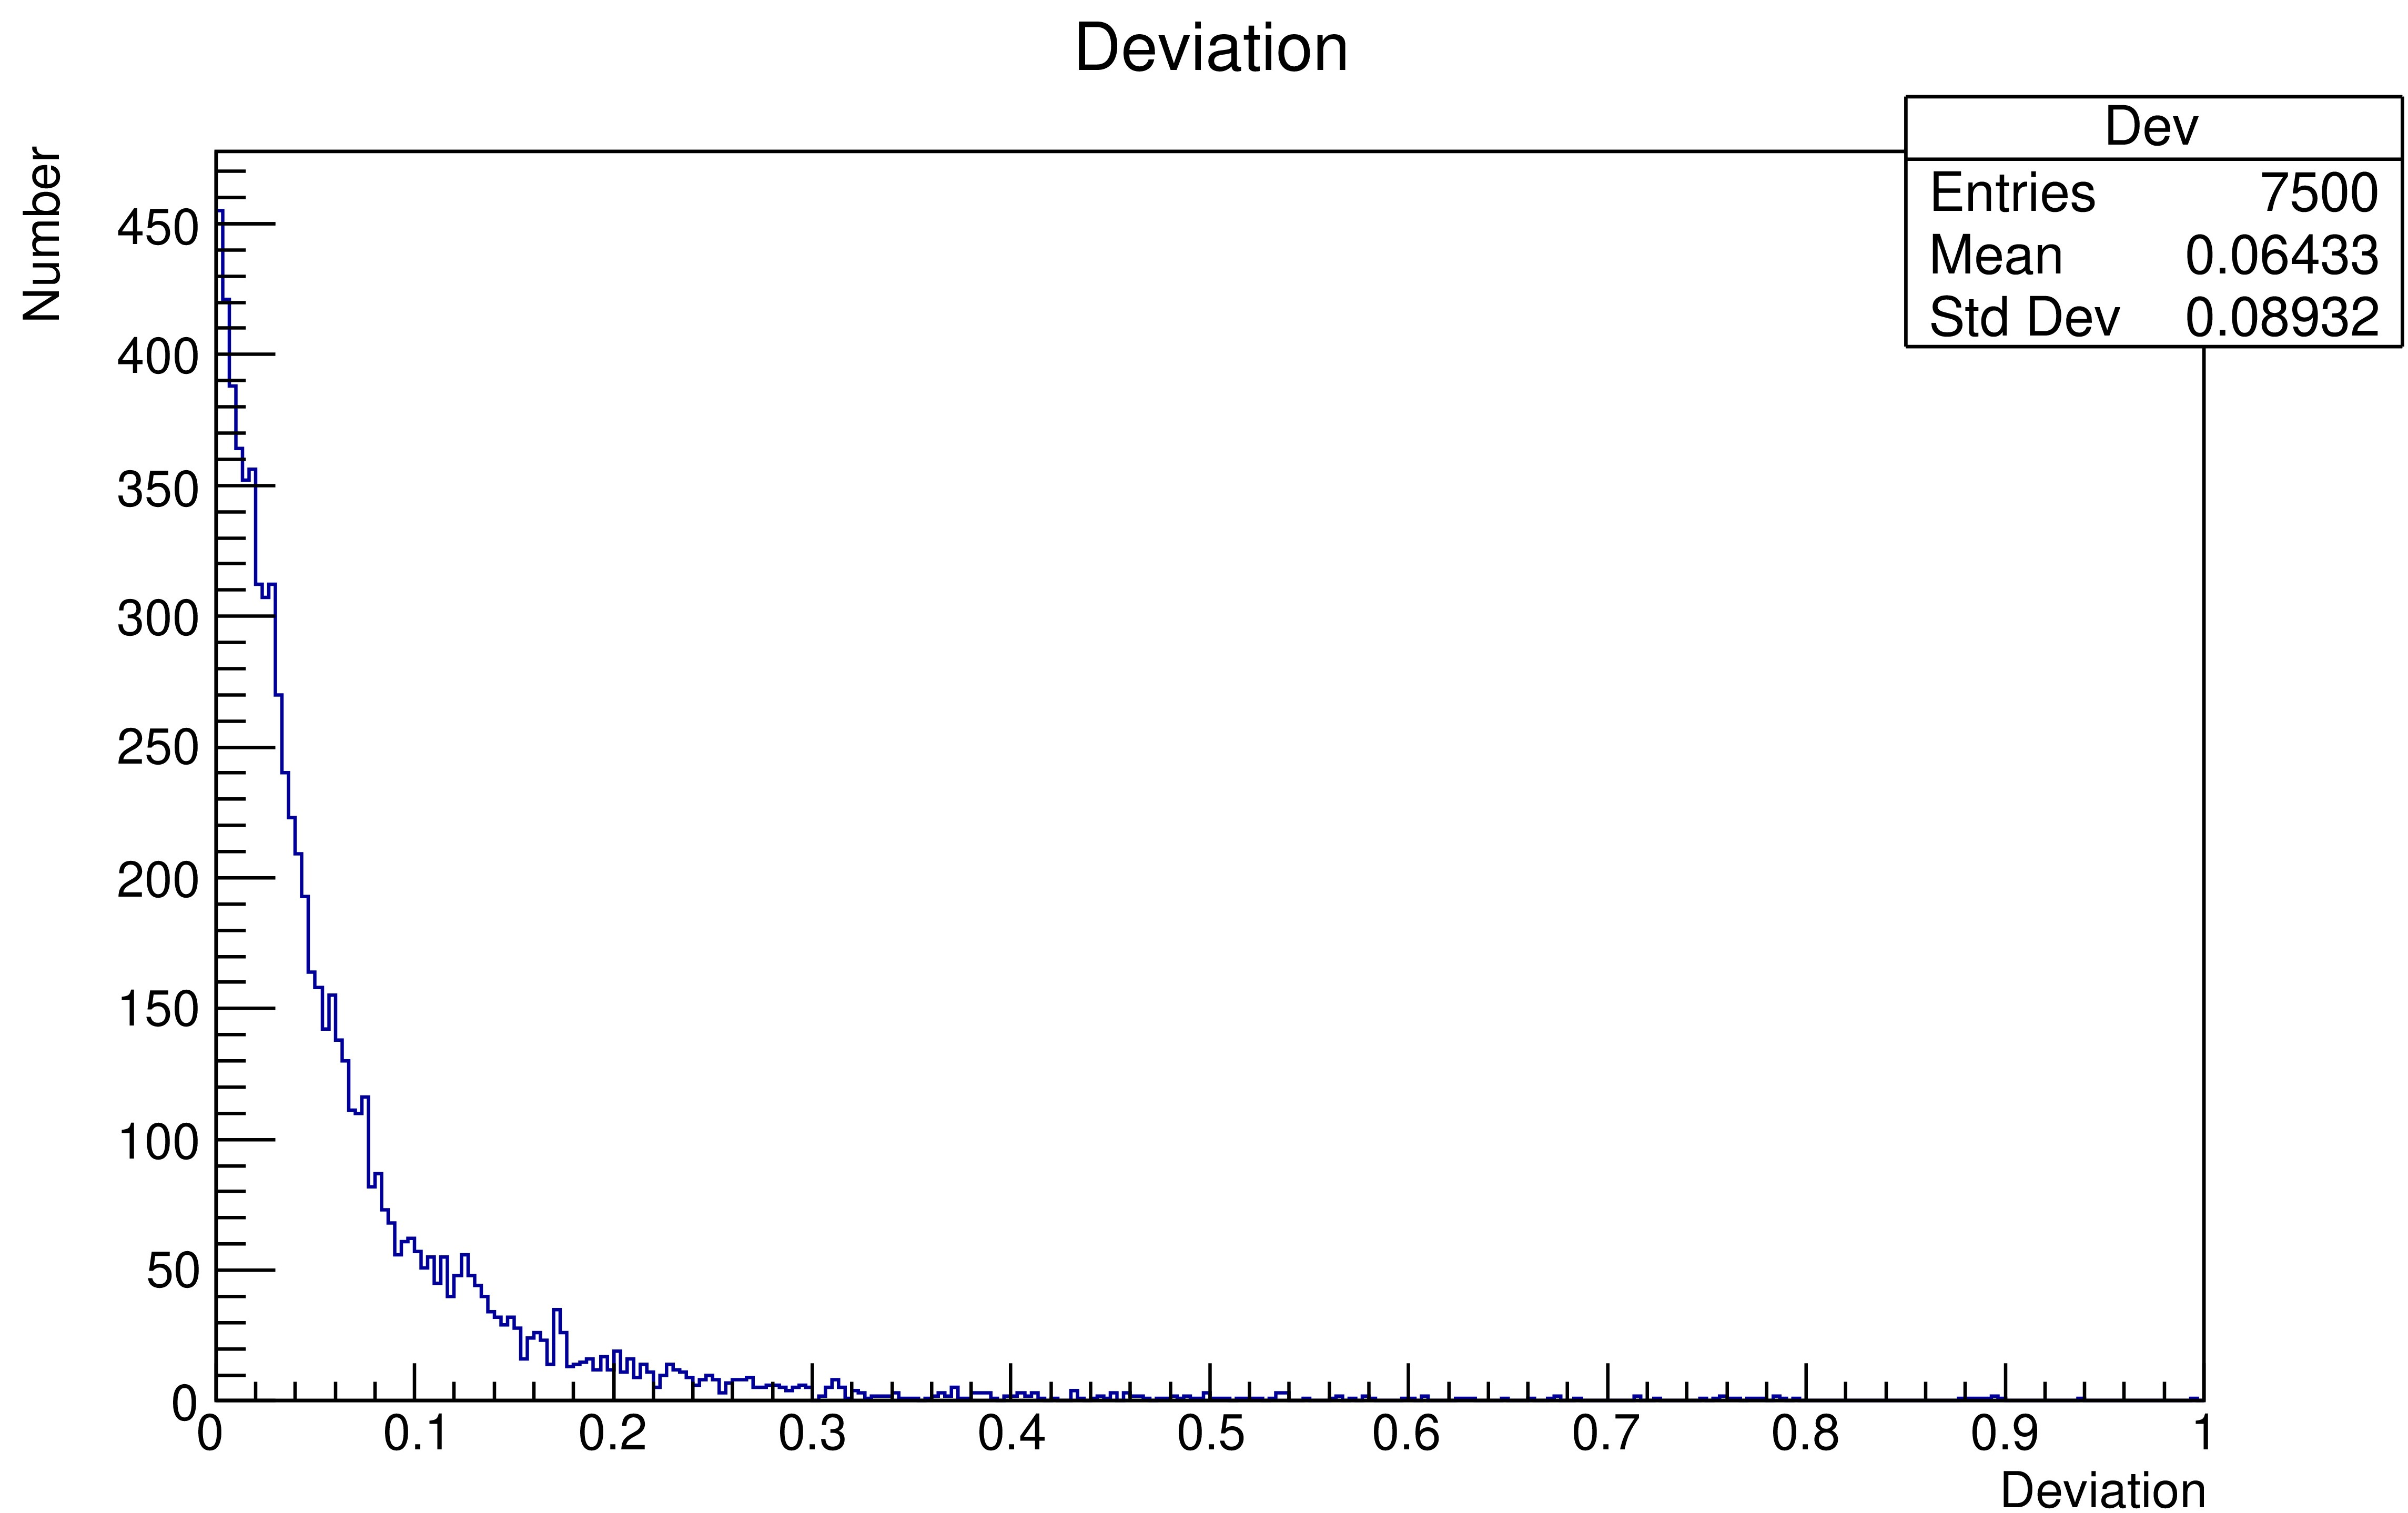
\includegraphics[width=0.32\textwidth]{figures/Deviation/Spine/SingleSourceUnshielded.jpg}\label{fig:exph7}}
%     \subfigure[克里金插值重构]{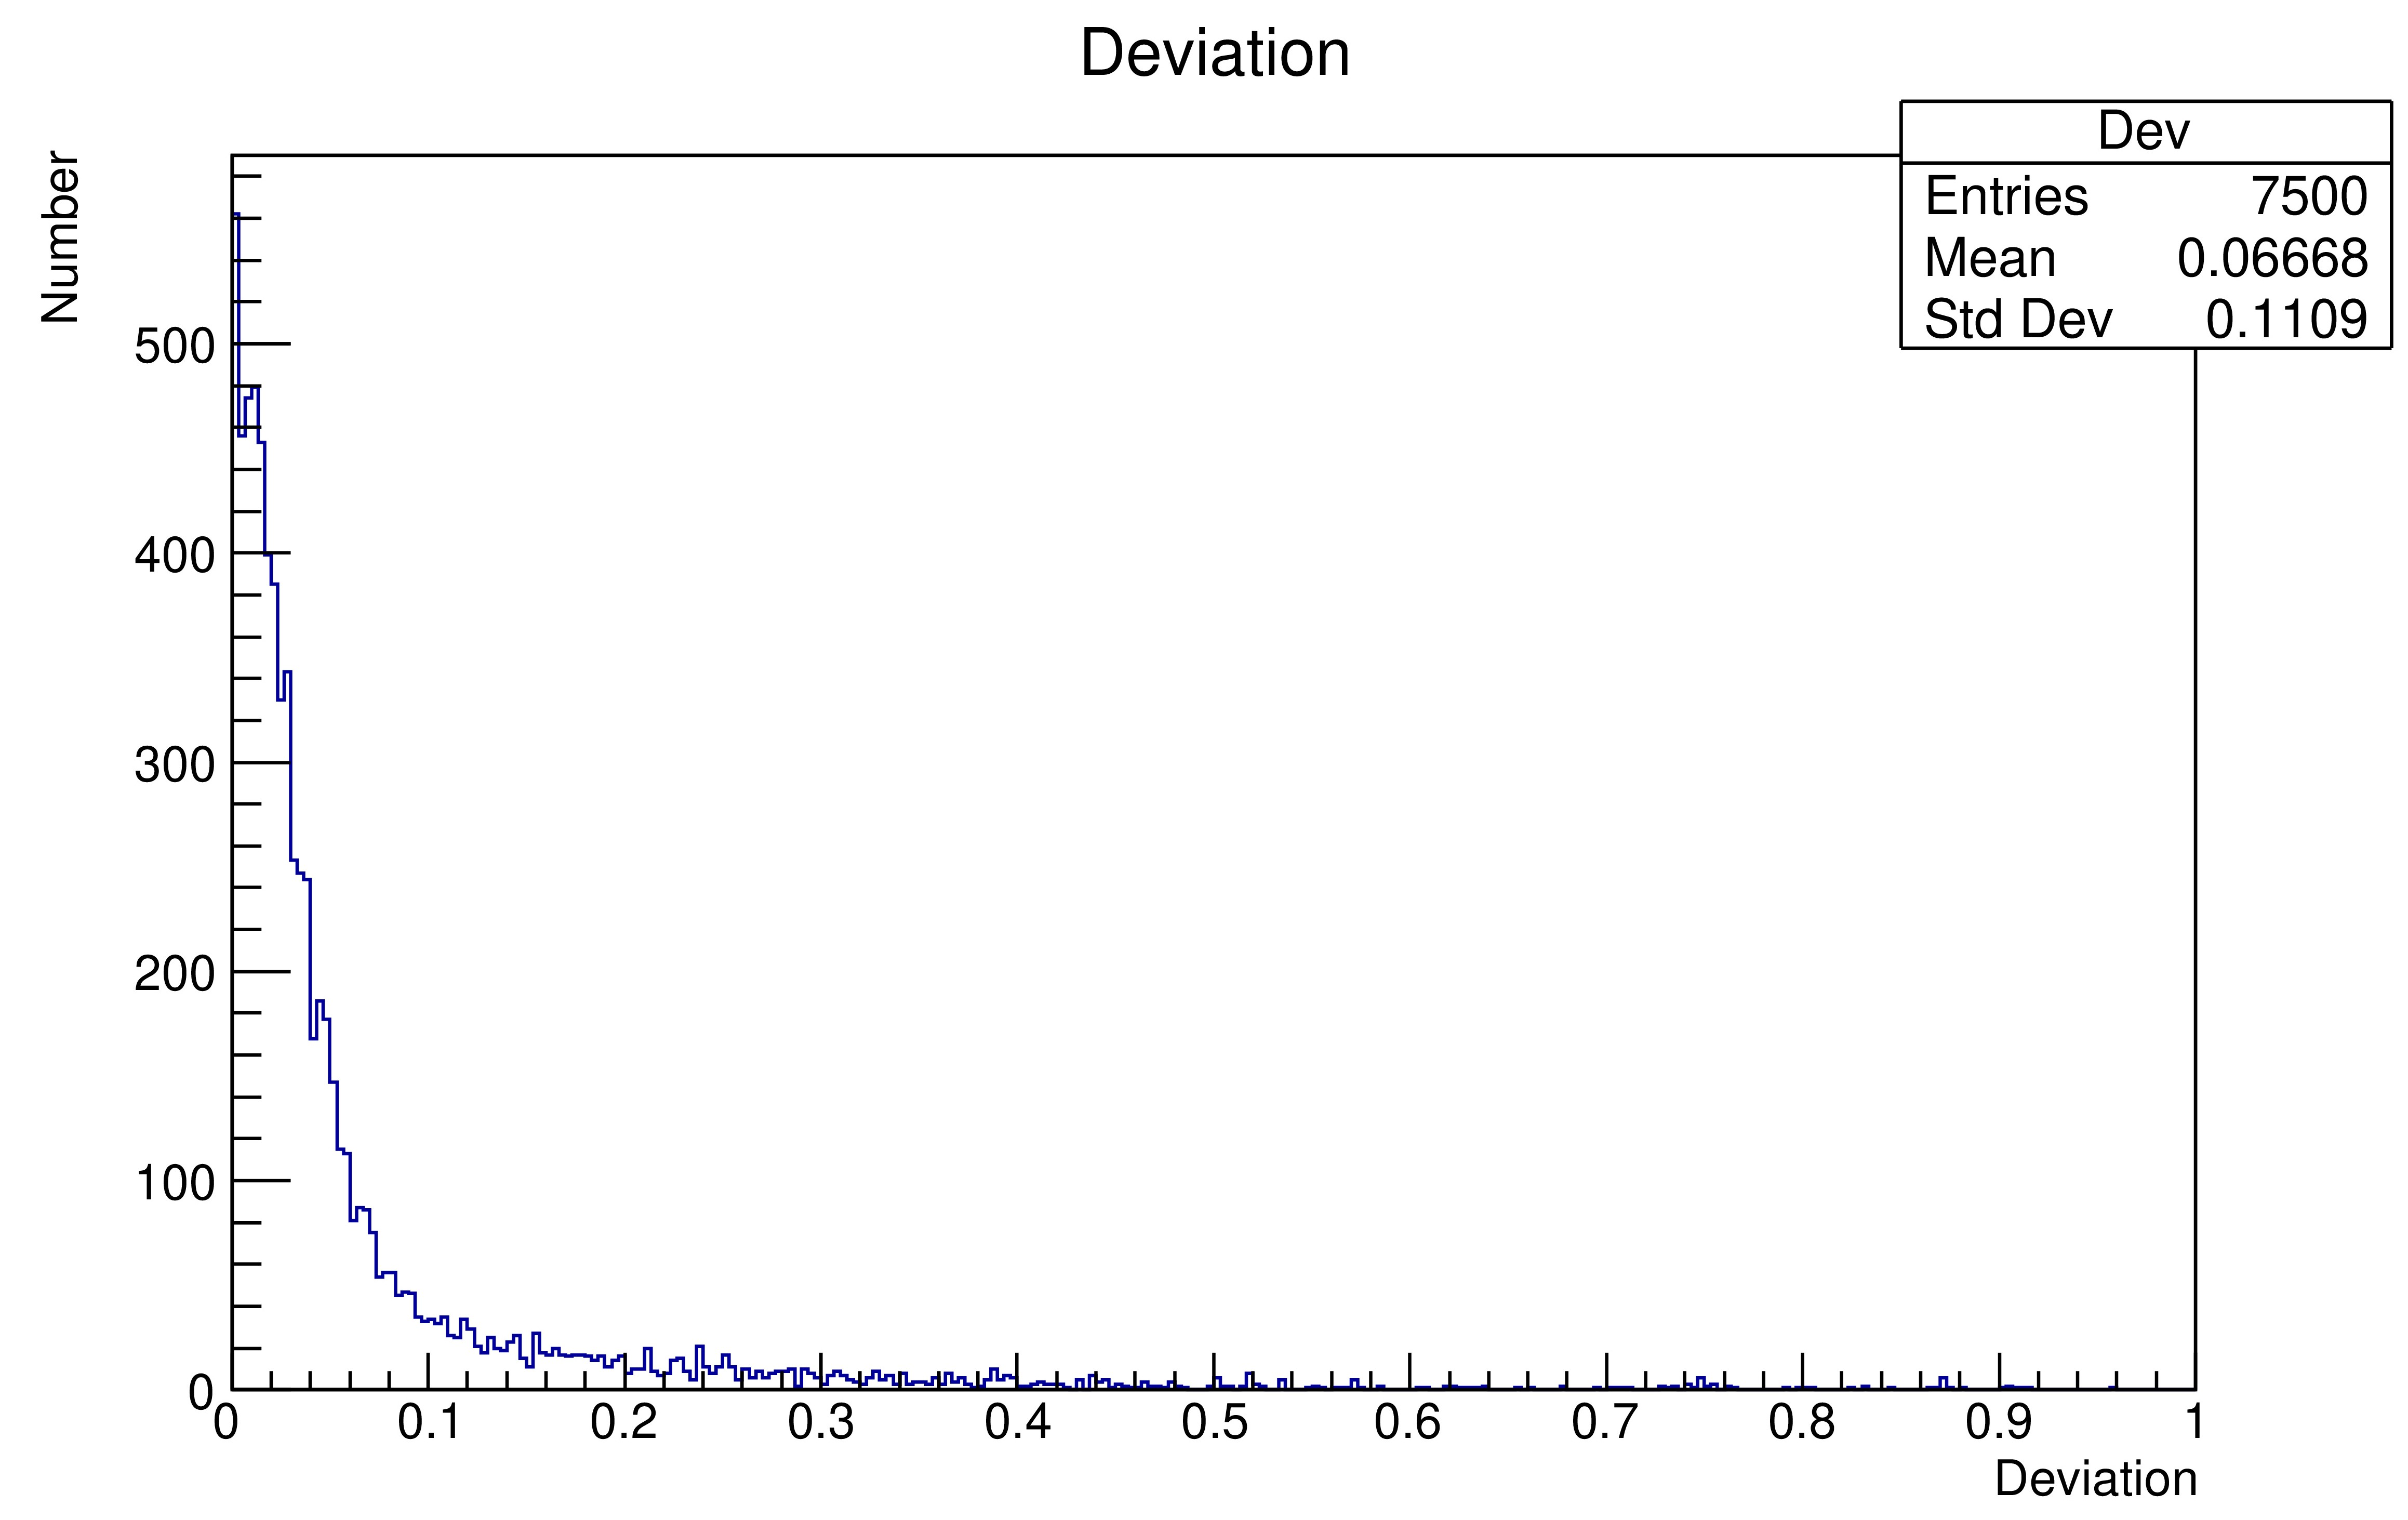
\includegraphics[width=0.32\textwidth]{figures/Deviation/Kriging/SingleSourceUnshielded.jpg}\label{fig:exgr7}}
%     \subfigure[创新插值重构]{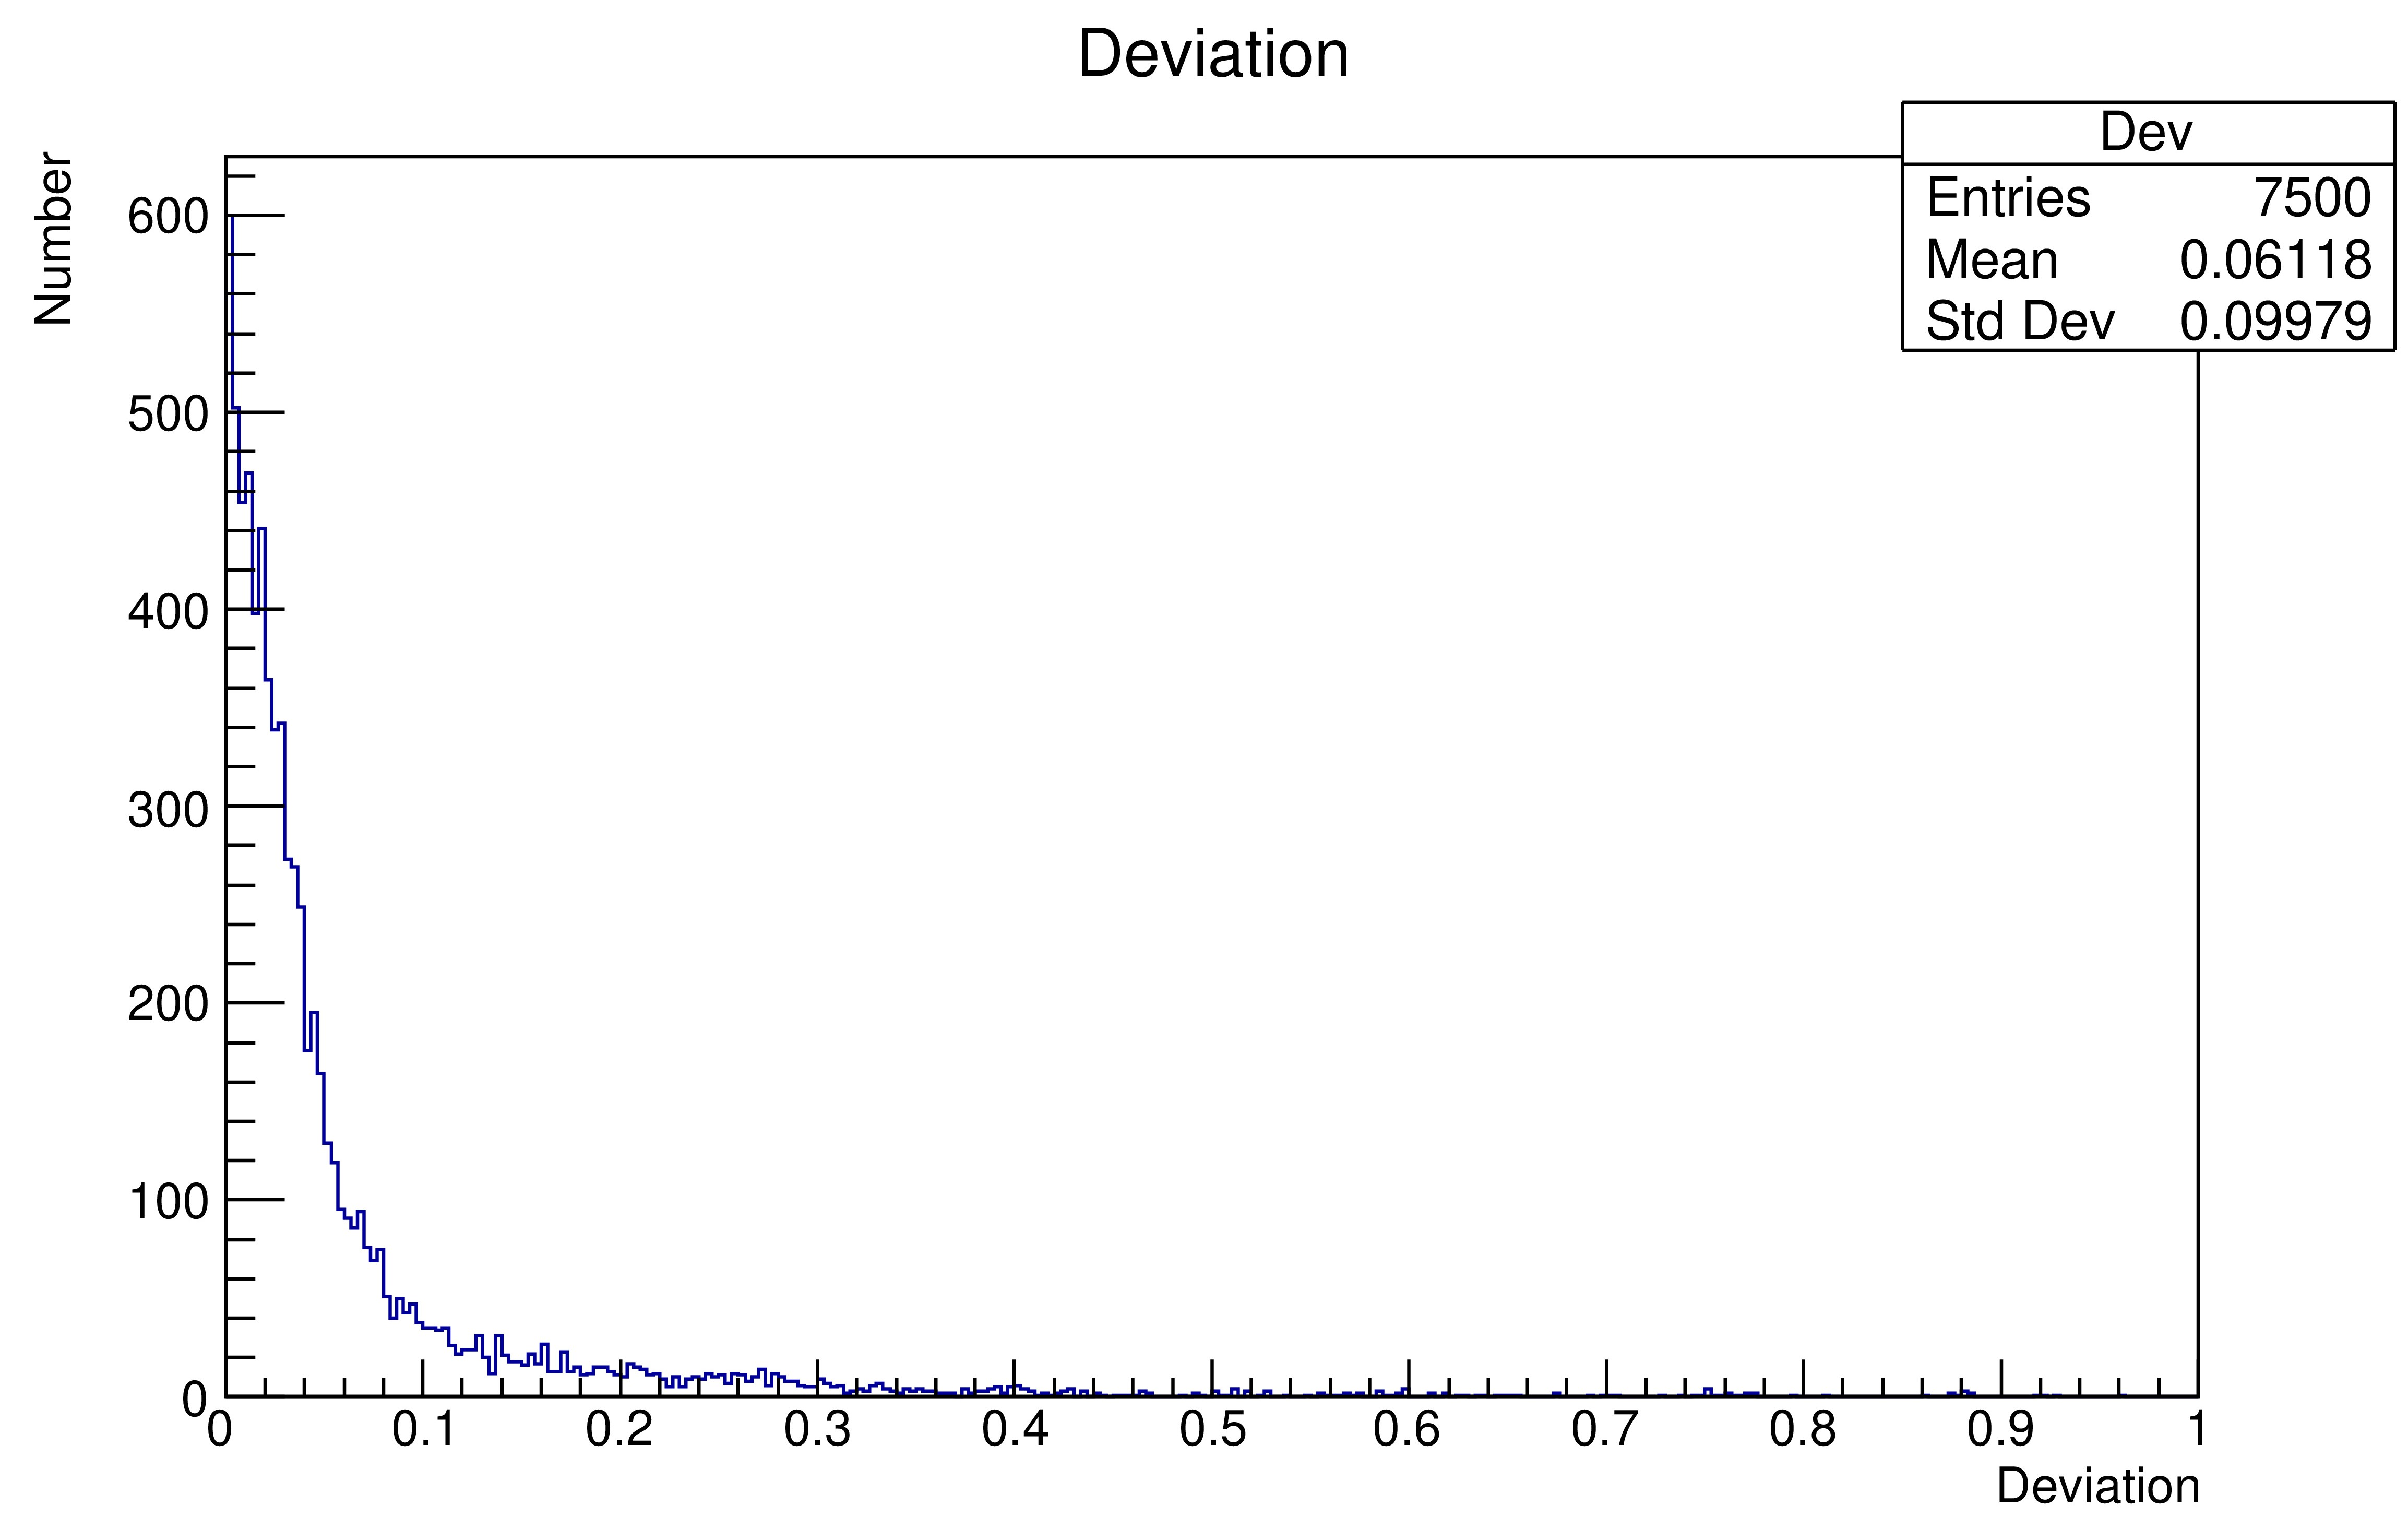
\includegraphics[width=0.32\textwidth]{figures/Deviation/RFRMethod/SingleSourceUnshielded.jpg}\label{fig:exls7}}
%     \caption{单点源无屏蔽空间辐射场插值重构相对偏差对比}
%     \label{单点源无屏蔽空间辐射场插值重构相对偏差对比}
% \end{figure}

% \begin{figure}[htbp]
%     \centering
%     \subfigure[多层B样条插值重构]{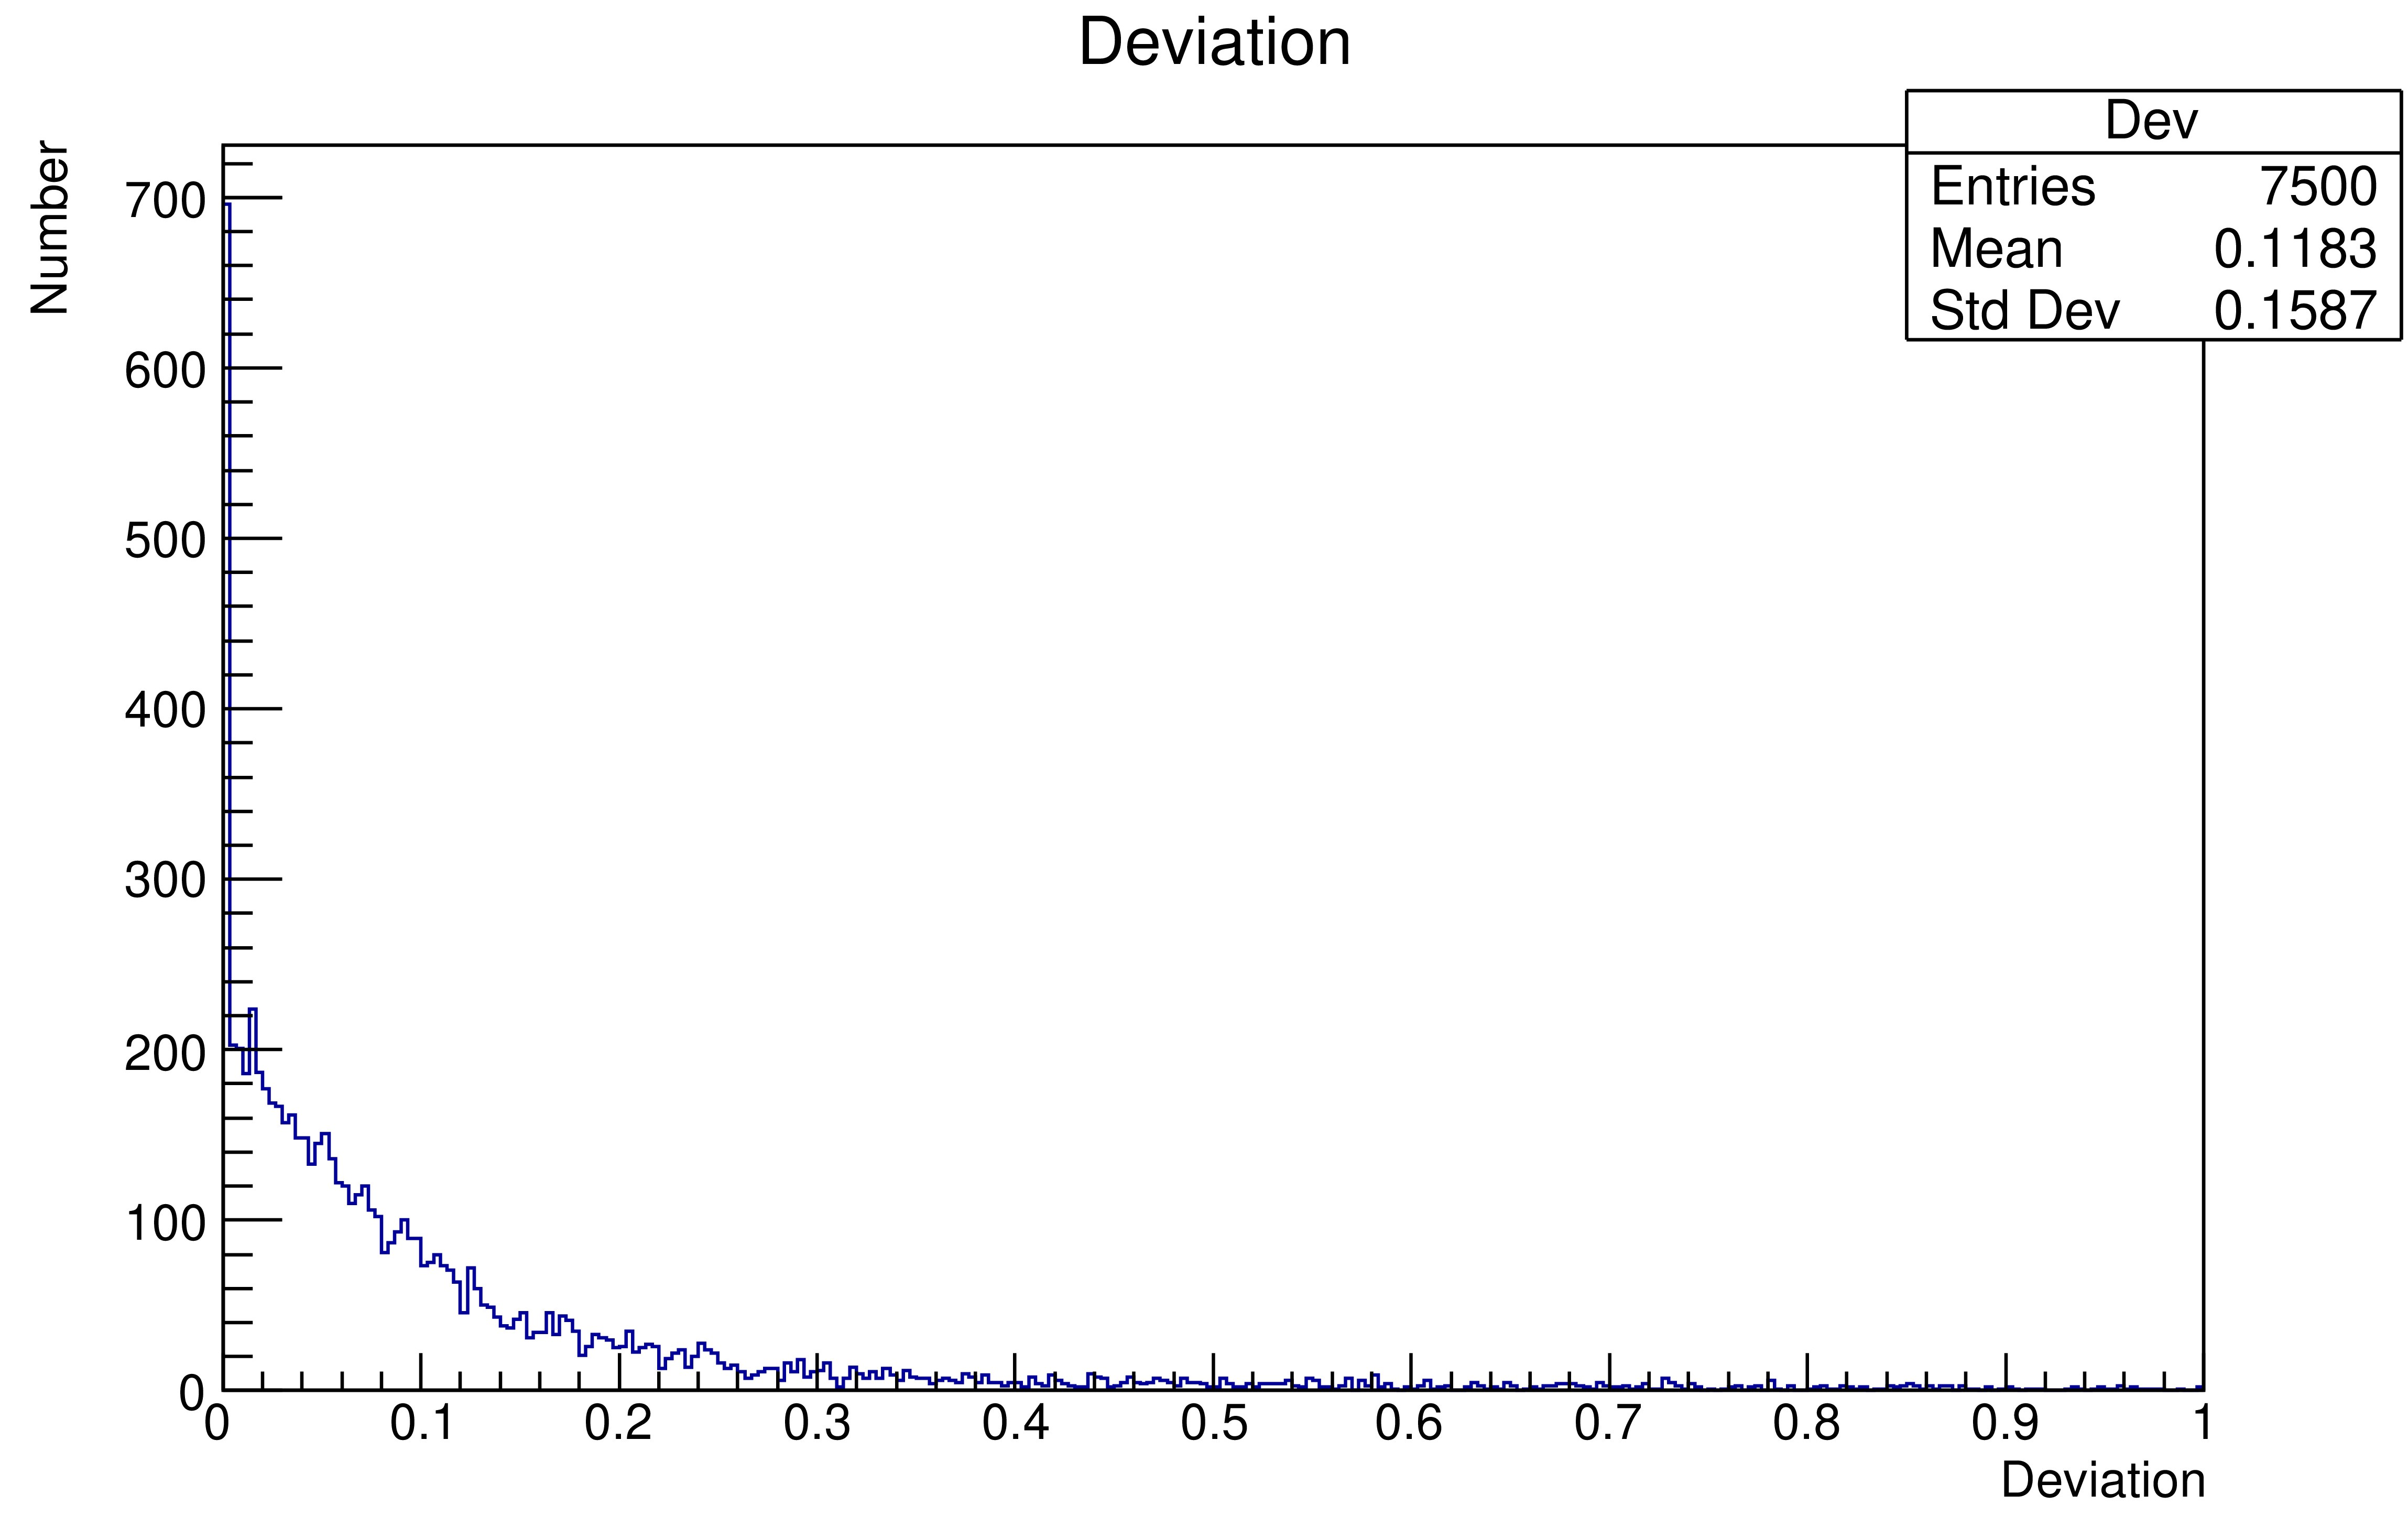
\includegraphics[width=0.32\textwidth]{figures/Deviation/Spine/MultiSourcesUnshielded.jpg}\label{fig:exph8}}
%     \subfigure[克里金插值重构]{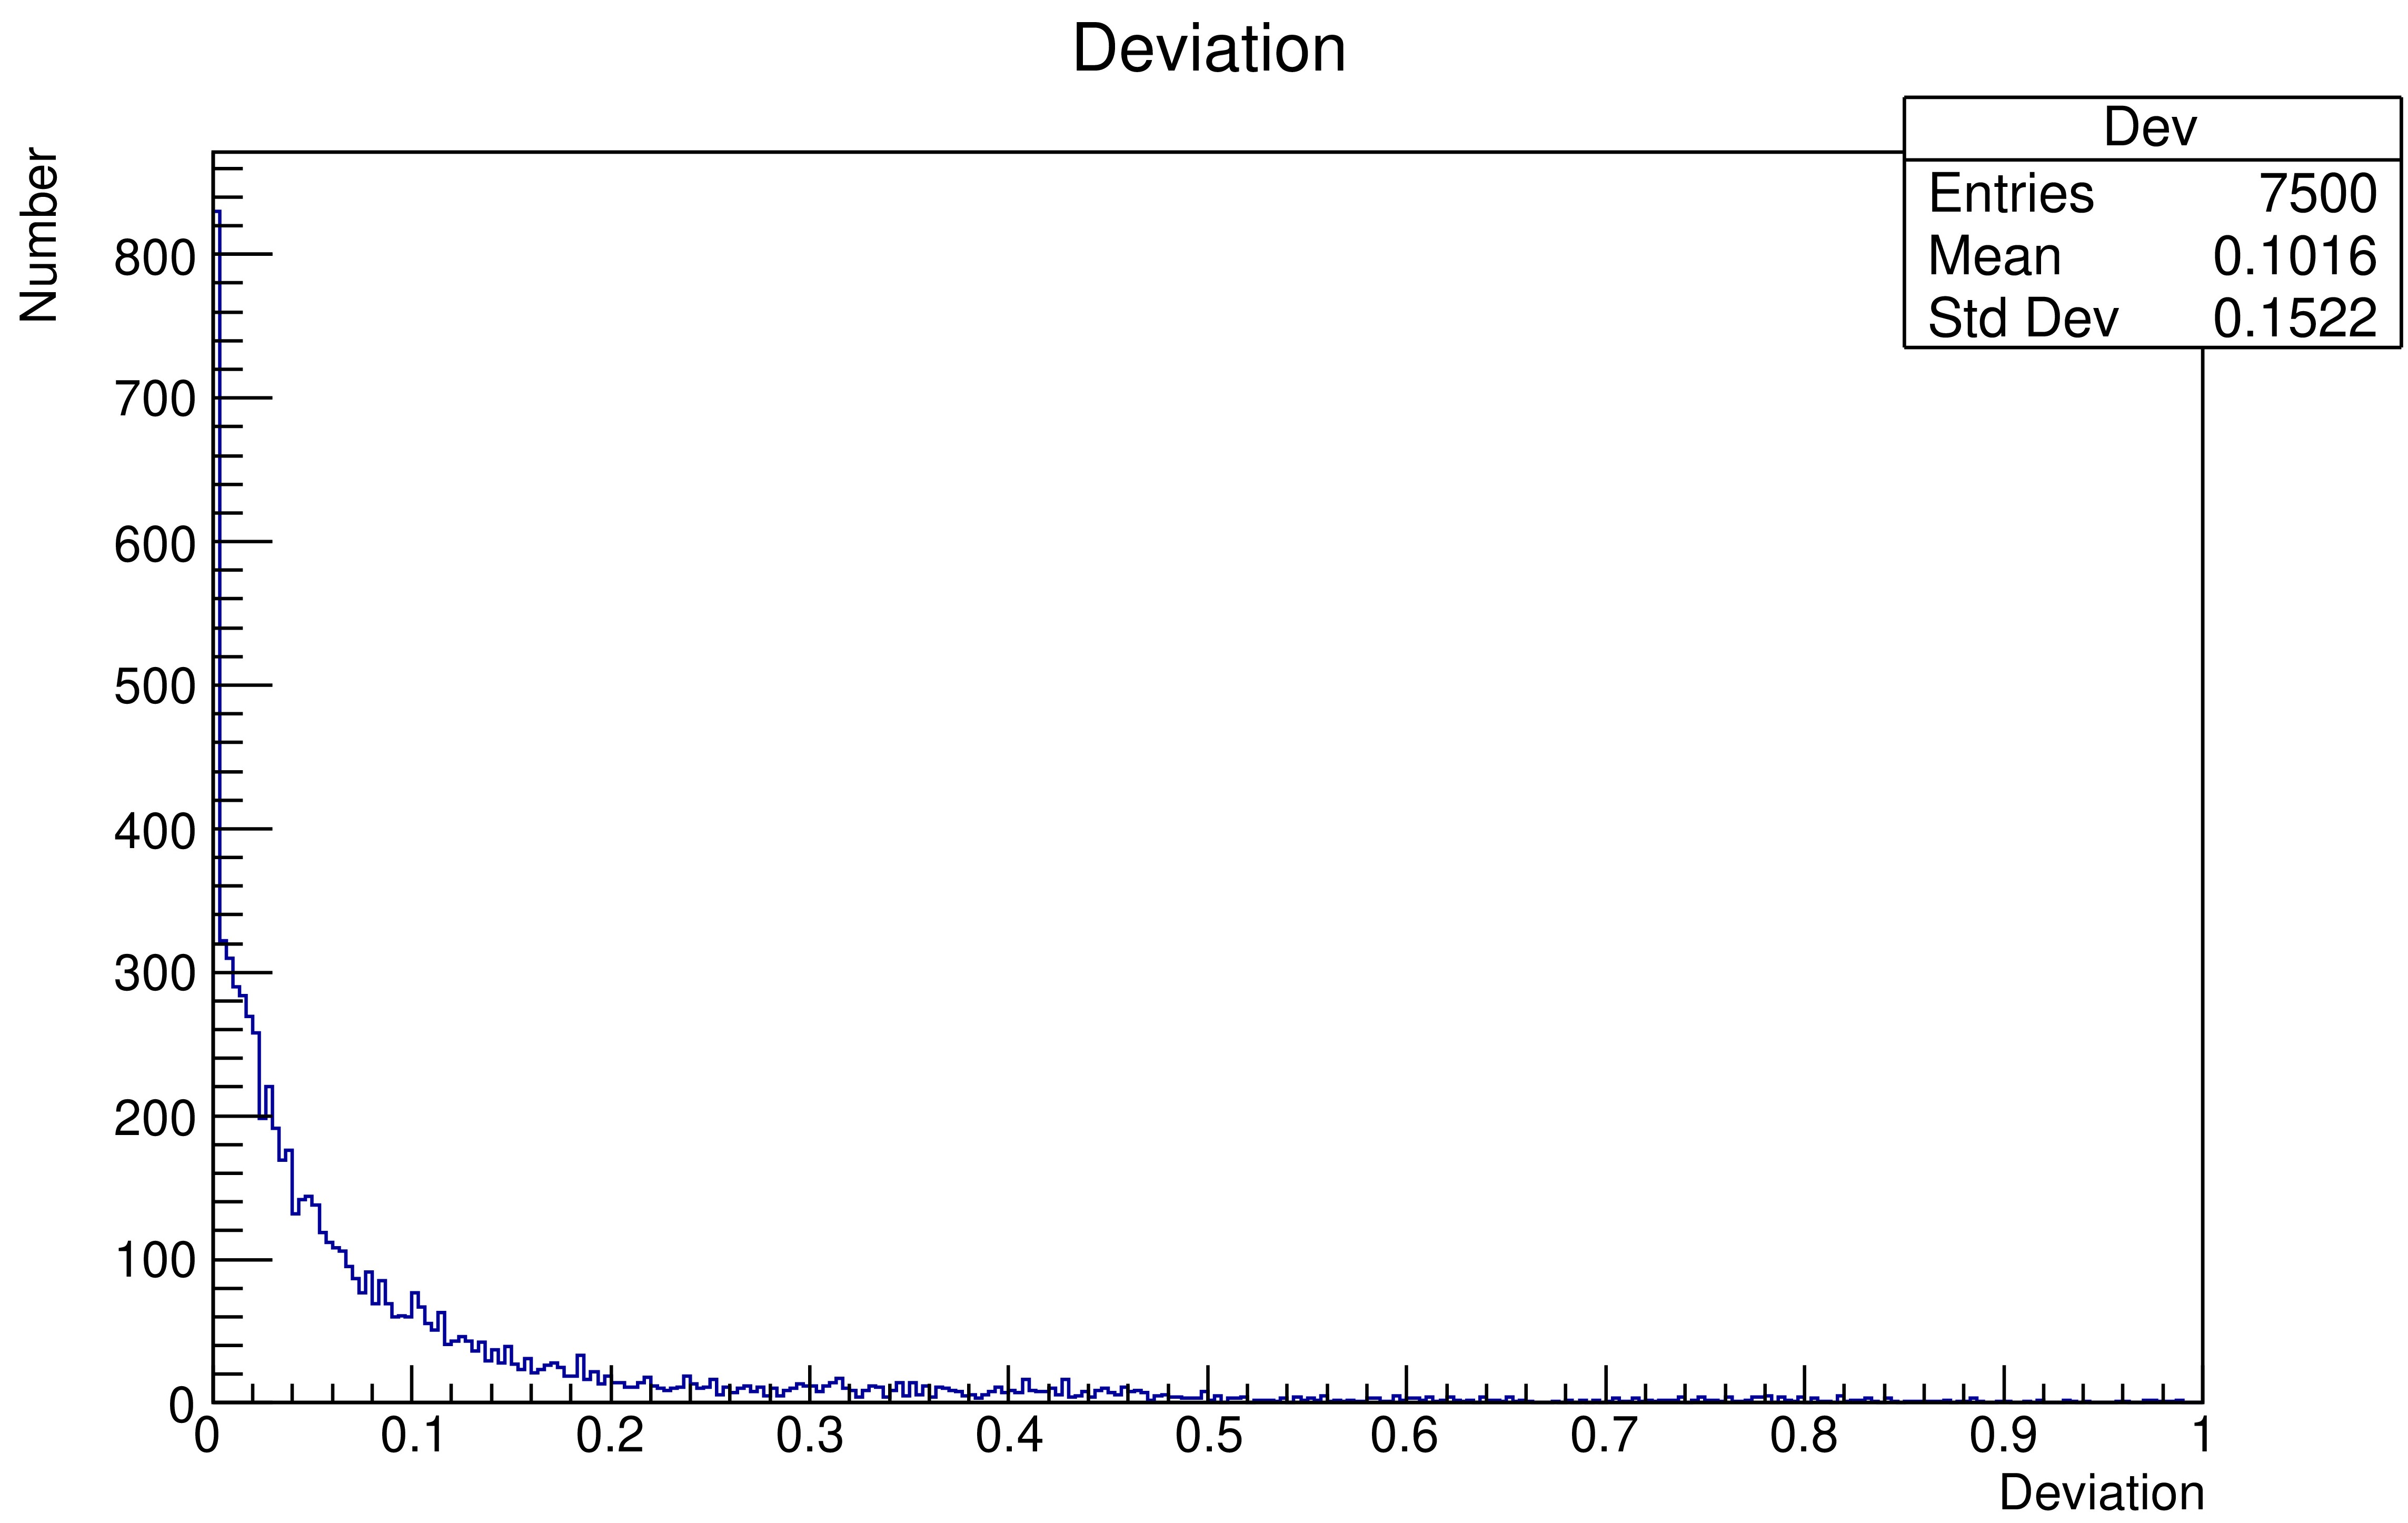
\includegraphics[width=0.32\textwidth]{figures/Deviation/Kriging/MultiSourcesUnshielded.jpg}\label{fig:exgr8}}
%     \subfigure[创新插值重构]{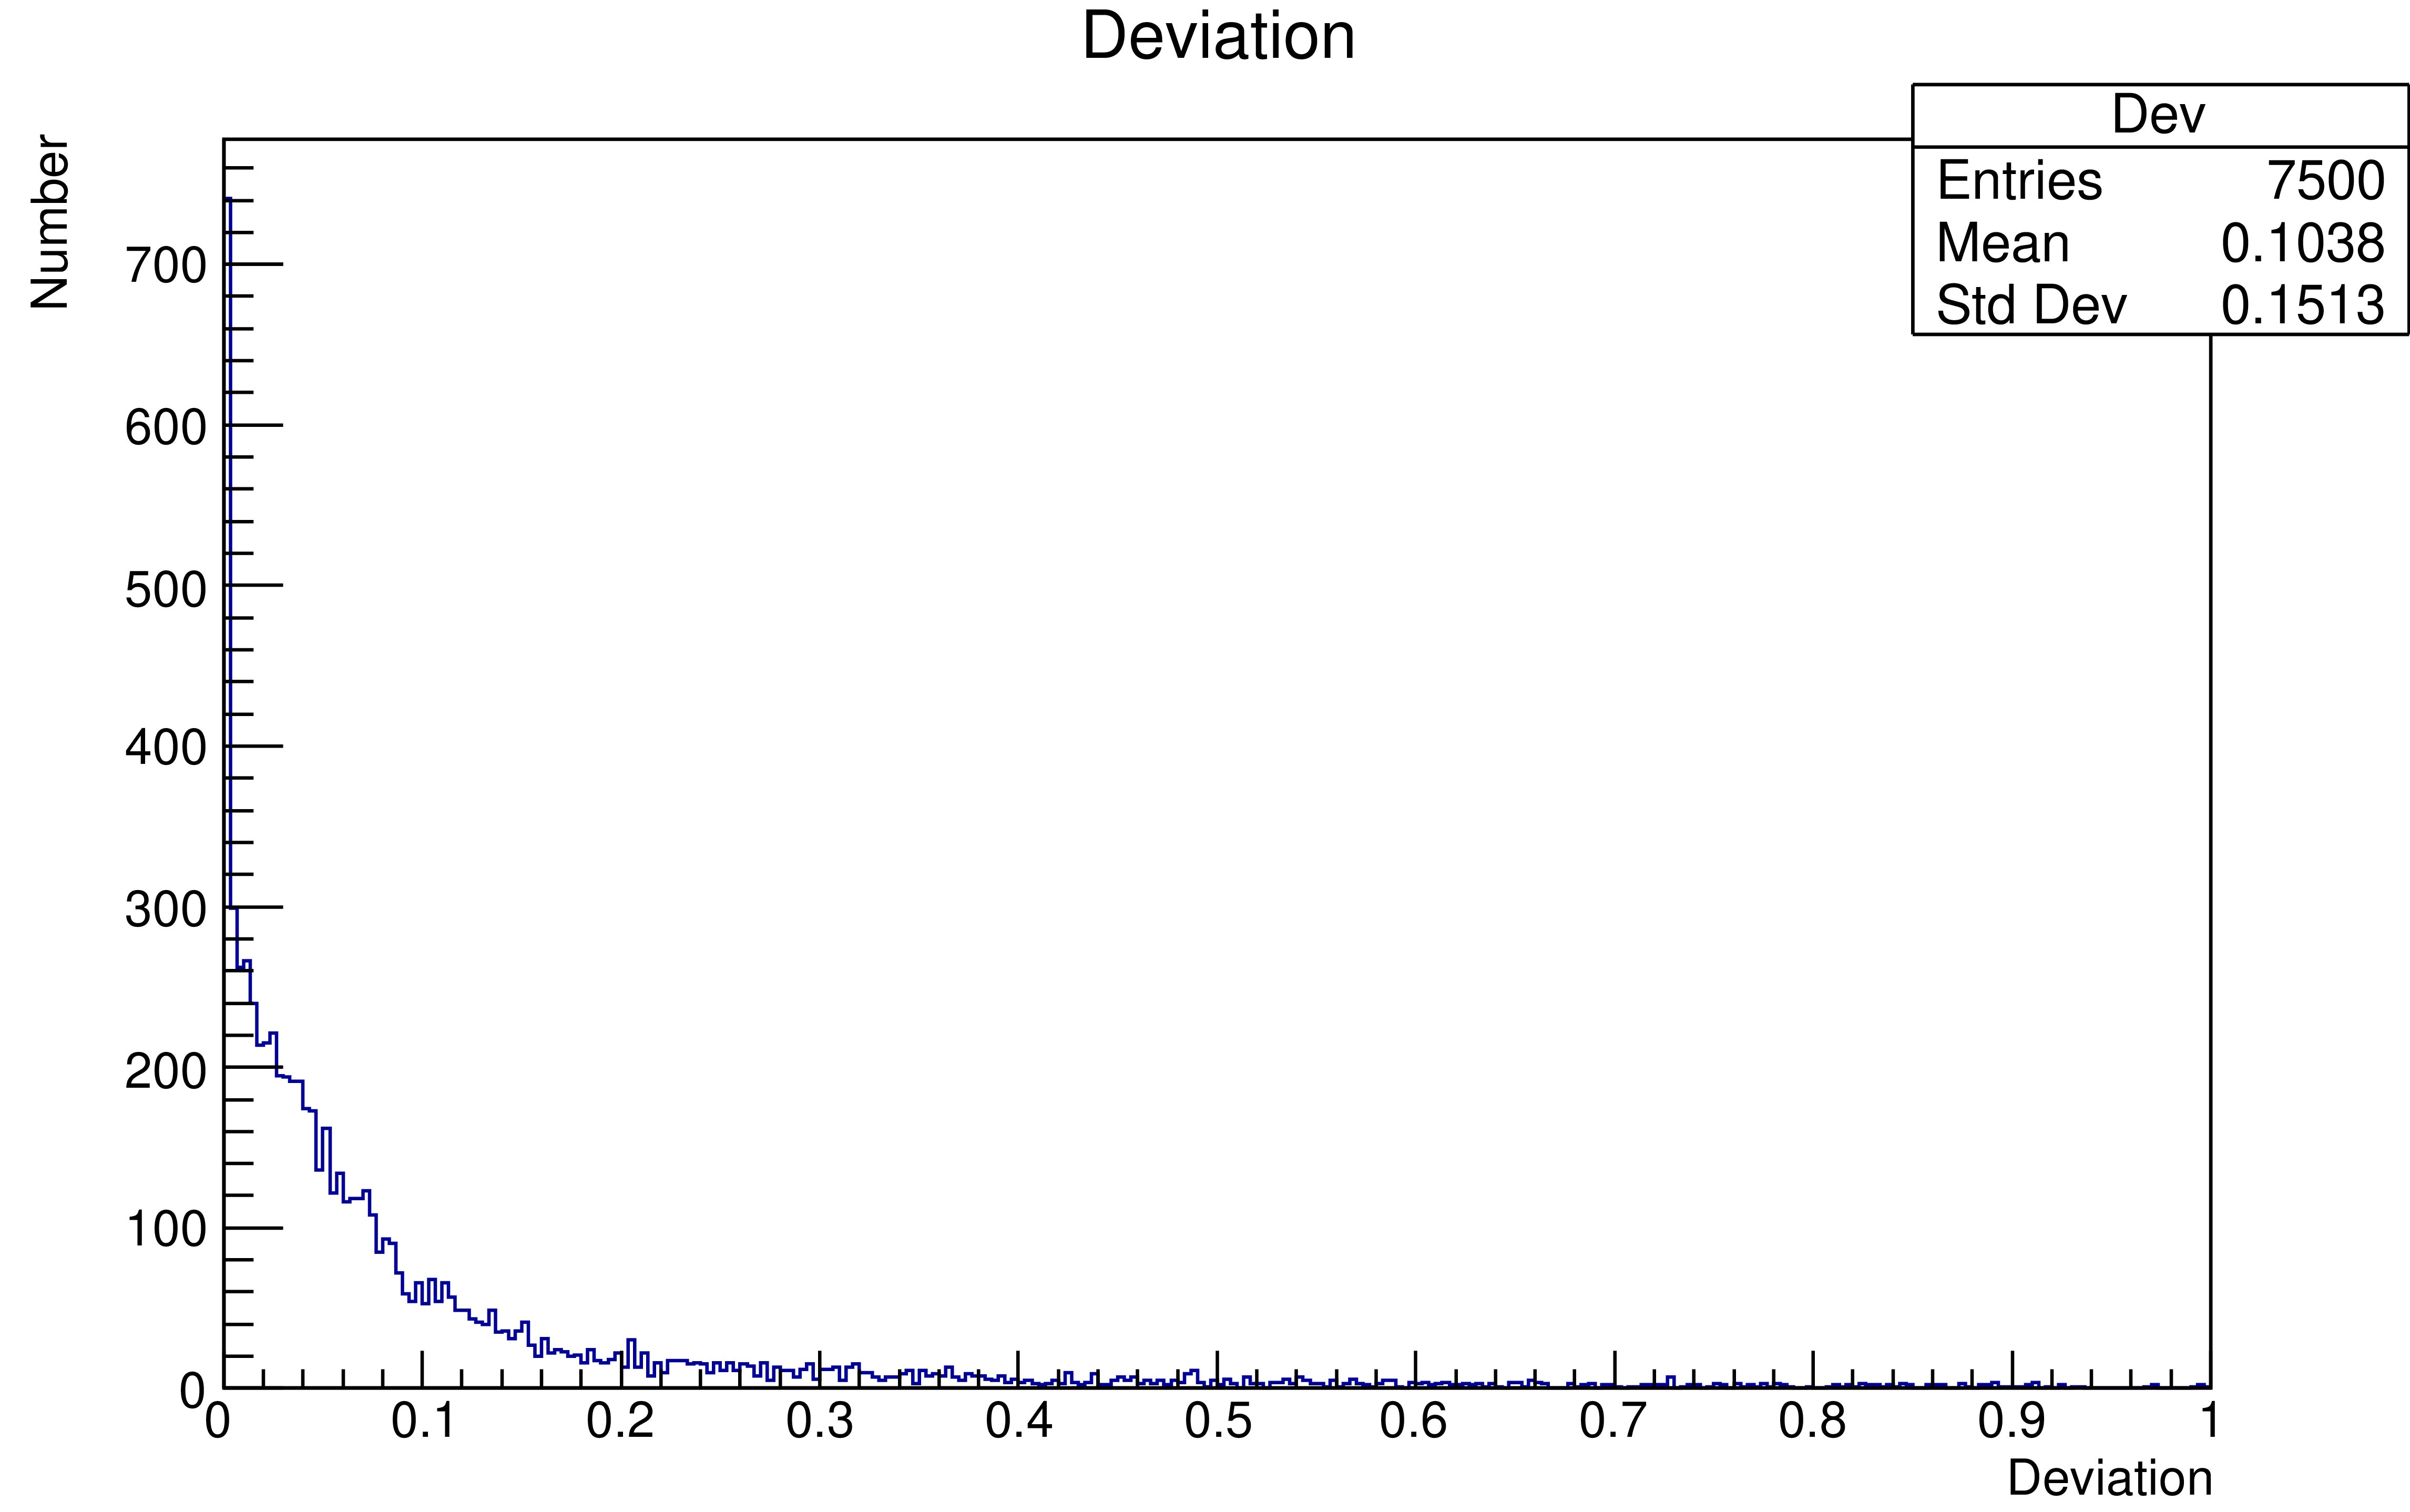
\includegraphics[width=0.32\textwidth]{figures/Deviation/RFRMethod/MultiSourcesUnshielded.jpg}\label{fig:exls8}}
%     \caption{多点源无屏蔽空间辐射场插值重构相对偏差对比}
%     \label{多点源无屏蔽空间辐射场插值重构相对偏差对比}
% \end{figure}

% \begin{figure}[htbp]
%     \centering
%     \subfigure[多层B样条插值重构]{\includegraphics[width=0.32\textwidth]{figures/Deviation/Spine/SingleSourceshielded.jpg}\label{fig:exph9}}
%     \subfigure[克里金插值重构]{\includegraphics[width=0.32\textwidth]{figures/Deviation/Kriging/SingleSourceshielded.jpg}\label{fig:exgr9}}
%     \subfigure[创新插值重构]{\includegraphics[width=0.32\textwidth]{figures/Deviation/RFRMethod/SingleSourceshielded.jpg}\label{fig:exls9}}
%     \caption{单点源有屏蔽空间辐射场插值重构相对偏差对比}
%     \label{单点源有屏蔽空间辐射场插值重构相对偏差对比}
% \end{figure}

\begin{figure}[htbp]
    \centering
    \subfigure[多层B样条插值重构]{\includegraphics[width=0.32\textwidth]{figures/Deviation/Spine/MultiSourcesshielded.jpg}\label{fig:exph10}}
    \subfigure[克里金插值重构]{\includegraphics[width=0.32\textwidth]{figures/Deviation/Kriging/MultiSourcesshielded.jpg}\label{fig:exgr10}}
    \subfigure[创新插值重构]{\includegraphics[width=0.32\textwidth]{figures/Deviation/RFRMethod/MultiSourcesshielded.jpg}\label{fig:exls10}}
    \caption{多点源有屏蔽空间辐射场插值重构相对偏差对比}
    \label{多点源有屏蔽空间辐射场插值重构相对偏差对比}
\end{figure}

\end{document}